\chapter{Risultati sperimentali}
\label{chp:risultati_nuovo}

I risultati sperimentali raccolti seguono la stessa progressione con cui è
stato costruito il lavoro. Si parte dalla verifica del
contesto sperimentale, cioè dal controllo empirico del dataset
\texttt{prefix\_constant\_rho} e dalla scelta di un seed stabile per gli
esperimenti successivi. Su questa base vengono poi confrontati gli algoritmi, 
osservando come evolve la stima lungo i prefissi e come
essa cambi al variare del rapporto tra elementi processati e distinti e del
parametro di precisione.

La seconda parte è dedicata al merge di sketch. Il punto di partenza è il caso
omogeneo, usato come controllo di correttezza dell'infrastruttura. Si passa poi
ai casi eterogenei, distinguendo tra situazioni \texttt{valid},
\texttt{invalid} e \texttt{recoverable}. Gli esperimenti su funzioni di hash
diverse e su mismatch di precisione servono da un lato a verificare quanto
emerso nella letteratura, dall'altro a mostrare che il framework costruito
consente di studiare in modo sistematico casi di merge non ideali.

\paragraph{Ambiente di test}
I risultati sono stati ottenuti su una workstation con processore AMD Ryzen 7
9700X, 32 GB di memoria DDR5 e unità a stato solido NVMe da 1 TB, con sistema
operativo CachyOS e ambiente grafico COSMIC.

La catena di compilazione utilizzata è:
\begin{itemize}[noitemsep]
    \item CMake 4.3.0;
    \item Clang 22.1.1;
    \item target \texttt{x86\_64-pc-linux-gnu}.
\end{itemize}

\section{Validazione del contesto sperimentale}

Prima di confrontare gli algoritmi è necessario verificare che il contesto di
prova sia coerente con le ipotesi alla base degli esperimenti successivi. La
sezione raccoglie quindi i controlli preliminari sul dataset utilizzato e sulla
scelta del seed mantenuto nelle esecuzioni principali.

\subsection{Verifica empirica del dataset a prefisso costante}

Gli esperimenti usano il dataset a prefisso costante con le seguenti configurazioni:
\[
n=10^7,\qquad p=50,\qquad seed=21041998,\qquad
d \in \{10^5,2\cdot 10^5,5\cdot 10^5,10^6,2\cdot 10^6,5\cdot 10^6,10^7\}
\]
\[
\rho=\frac{n}{d}\in\{100,50,20,10,5,2,1\}
\]
I sette valori di \(\rho\) corrispondono ai rapporti tra elementi processati e
distinti usati nel resto del capitolo.

La validazione empirica del comportamento del dataset è mostrata nelle
Figure~\ref{fig:ch5-dataset-rho-ratio-linear} e
\ref{fig:ch5-dataset-rho-ratio-boundary}.
La prima figura mostra il rapporto \(\rho_t=t/F_0(t)\) sui punti di controllo
effettivamente usati nella modalità di flusso, mentre la seconda isola i soli
punti di bordo dei blocchi, nei quali il rapporto assume il valore costante
previsto dalla costruzione.

Dalle figure si osserva che il comportamento atteso è rispettato. All'interno
  di ciascun blocco la cardinalità distinta non cresce, perché non vengono
  introdotte nuove prime occorrenze, mentre ai bordi di blocco essa aumenta di una
  sola unità. Ne segue che il rapporto \(\rho_t=t/F_0(t)\) assume il valore
  teorico \(\rho\) esattamente nei punti \(t=j\cdot\rho\), in accordo con la
  costruzione del dataset.

\begin{figure}[htbp]
    \centering
    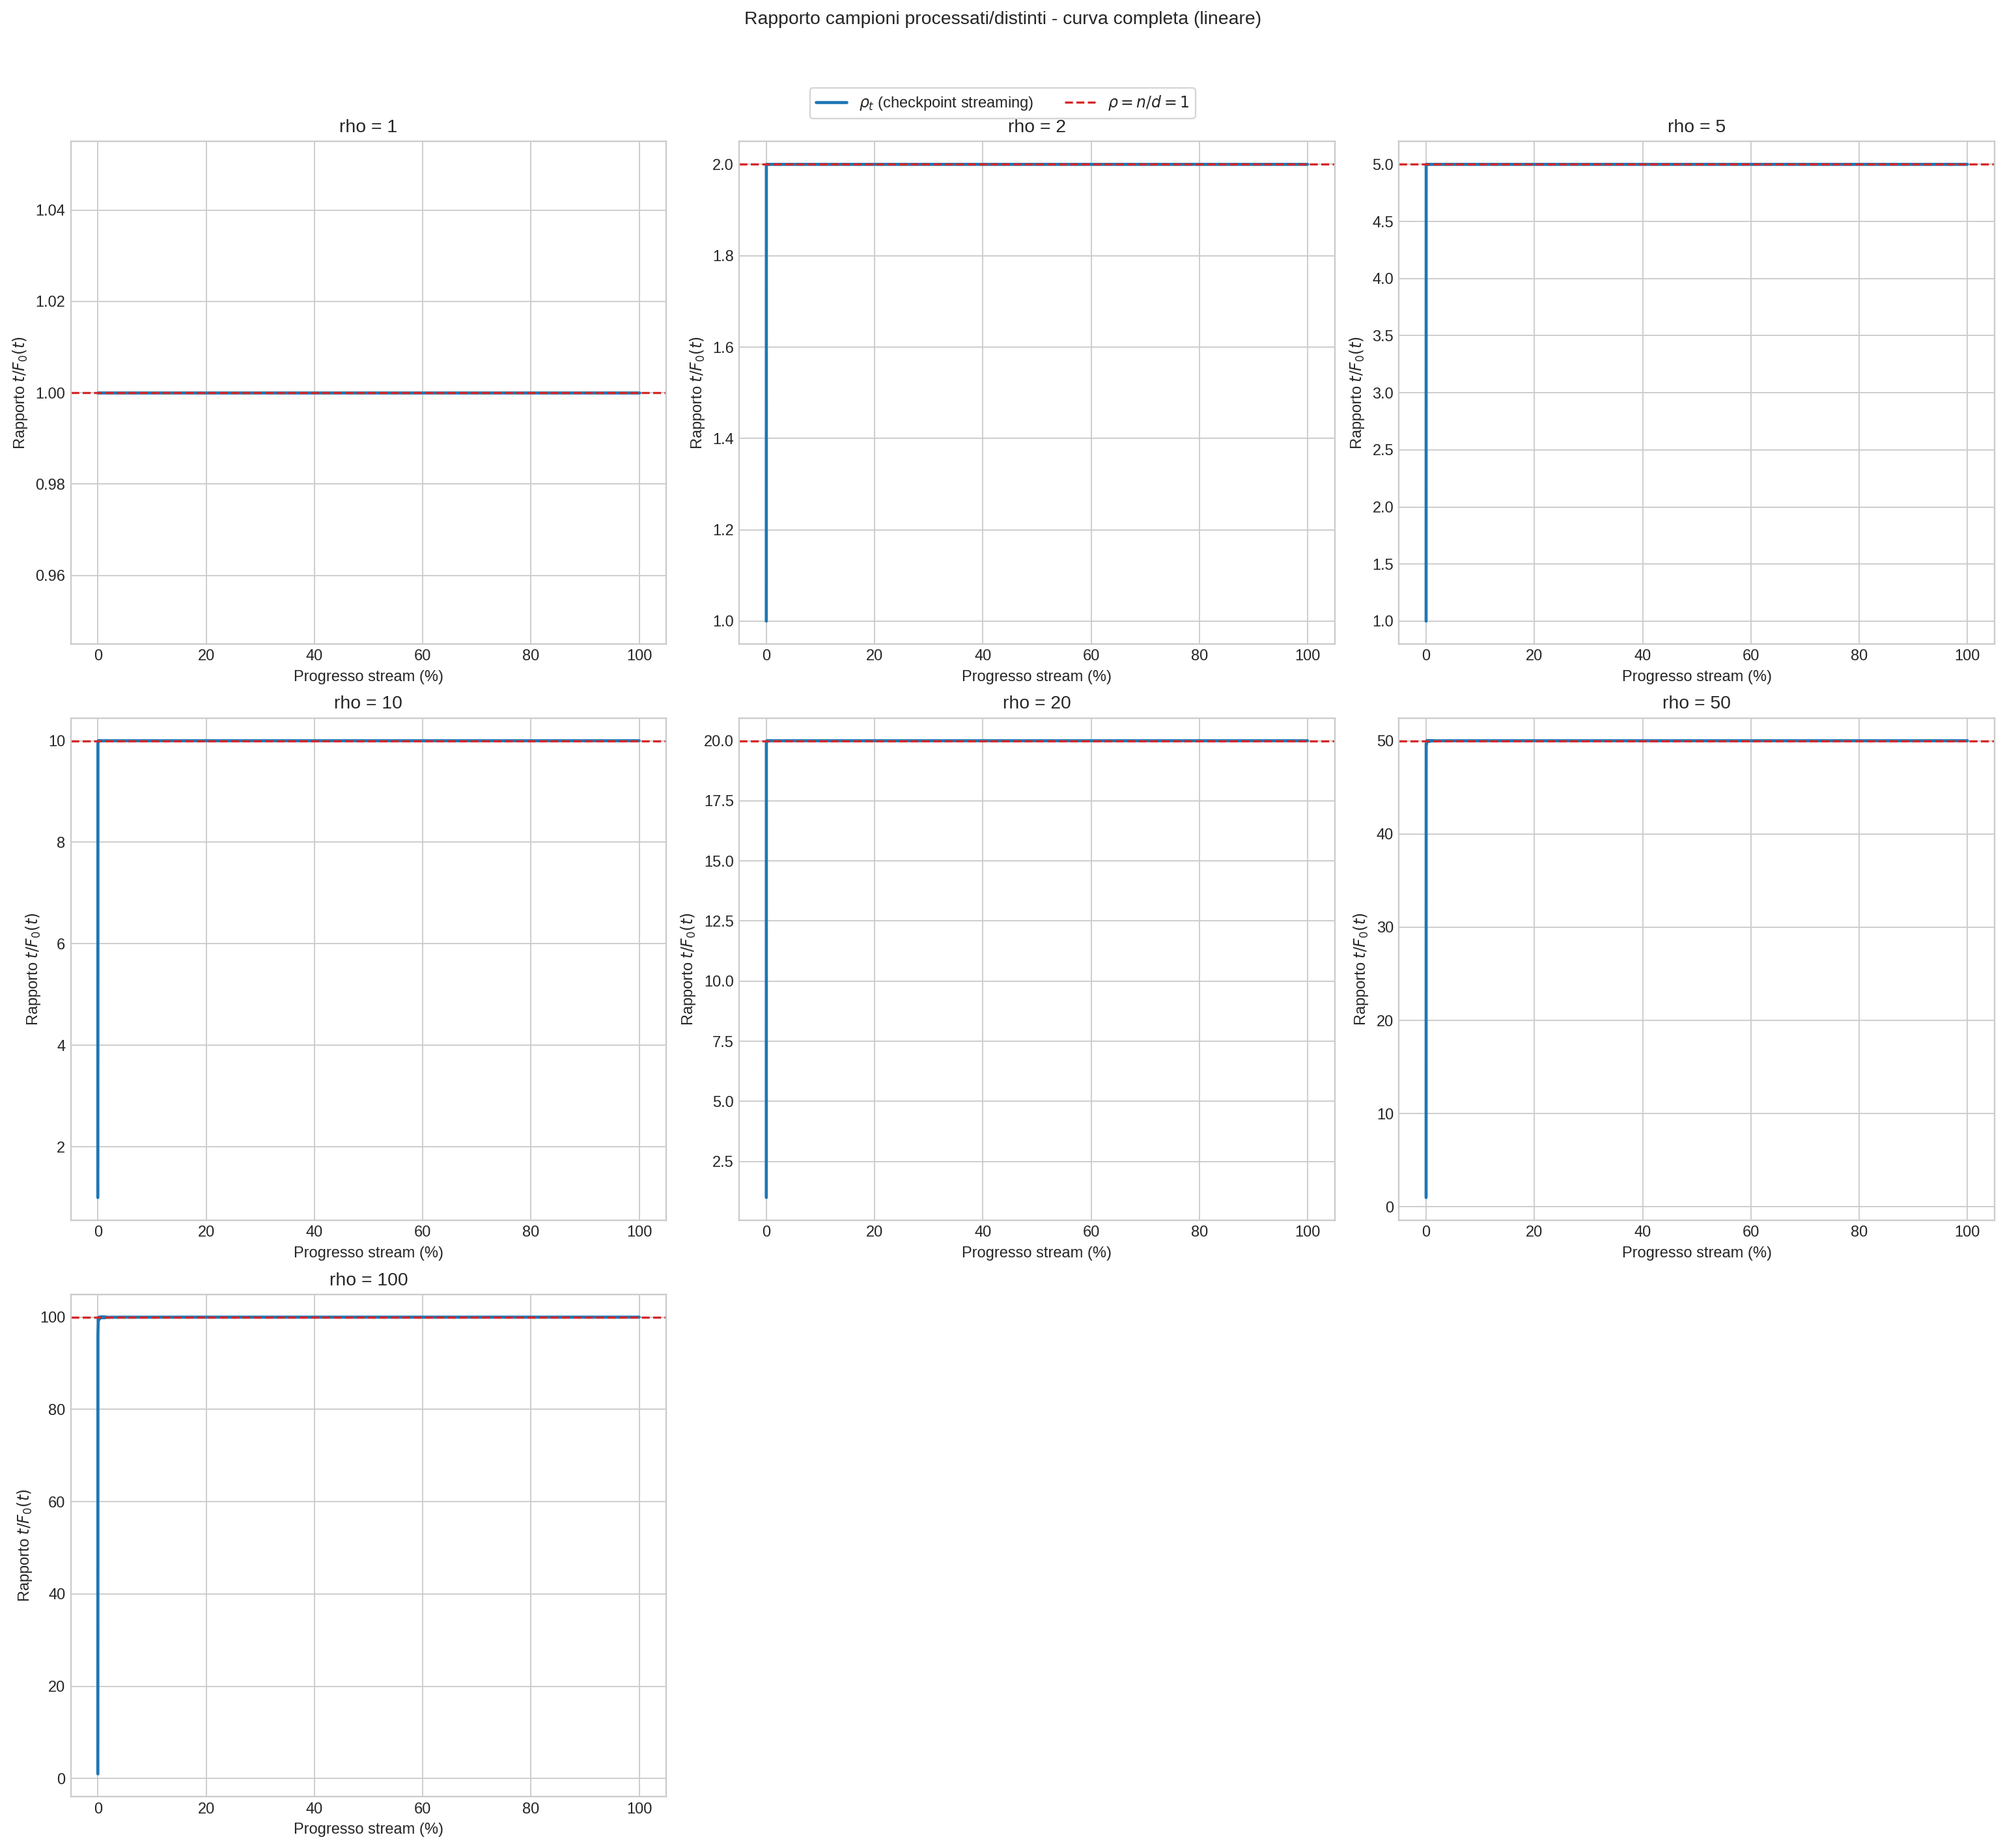
\includegraphics[width=0.96\textwidth]{figures/results/ratio_processed_vs_distinct_streaming_linear.png}
    \caption{Rapporto \(\rho_t=t/F_0(t)\) osservato ai checkpoint del dataset}
    \label{fig:ch5-dataset-rho-ratio-linear}
\end{figure}

\begin{figure}[htbp]
    \centering
    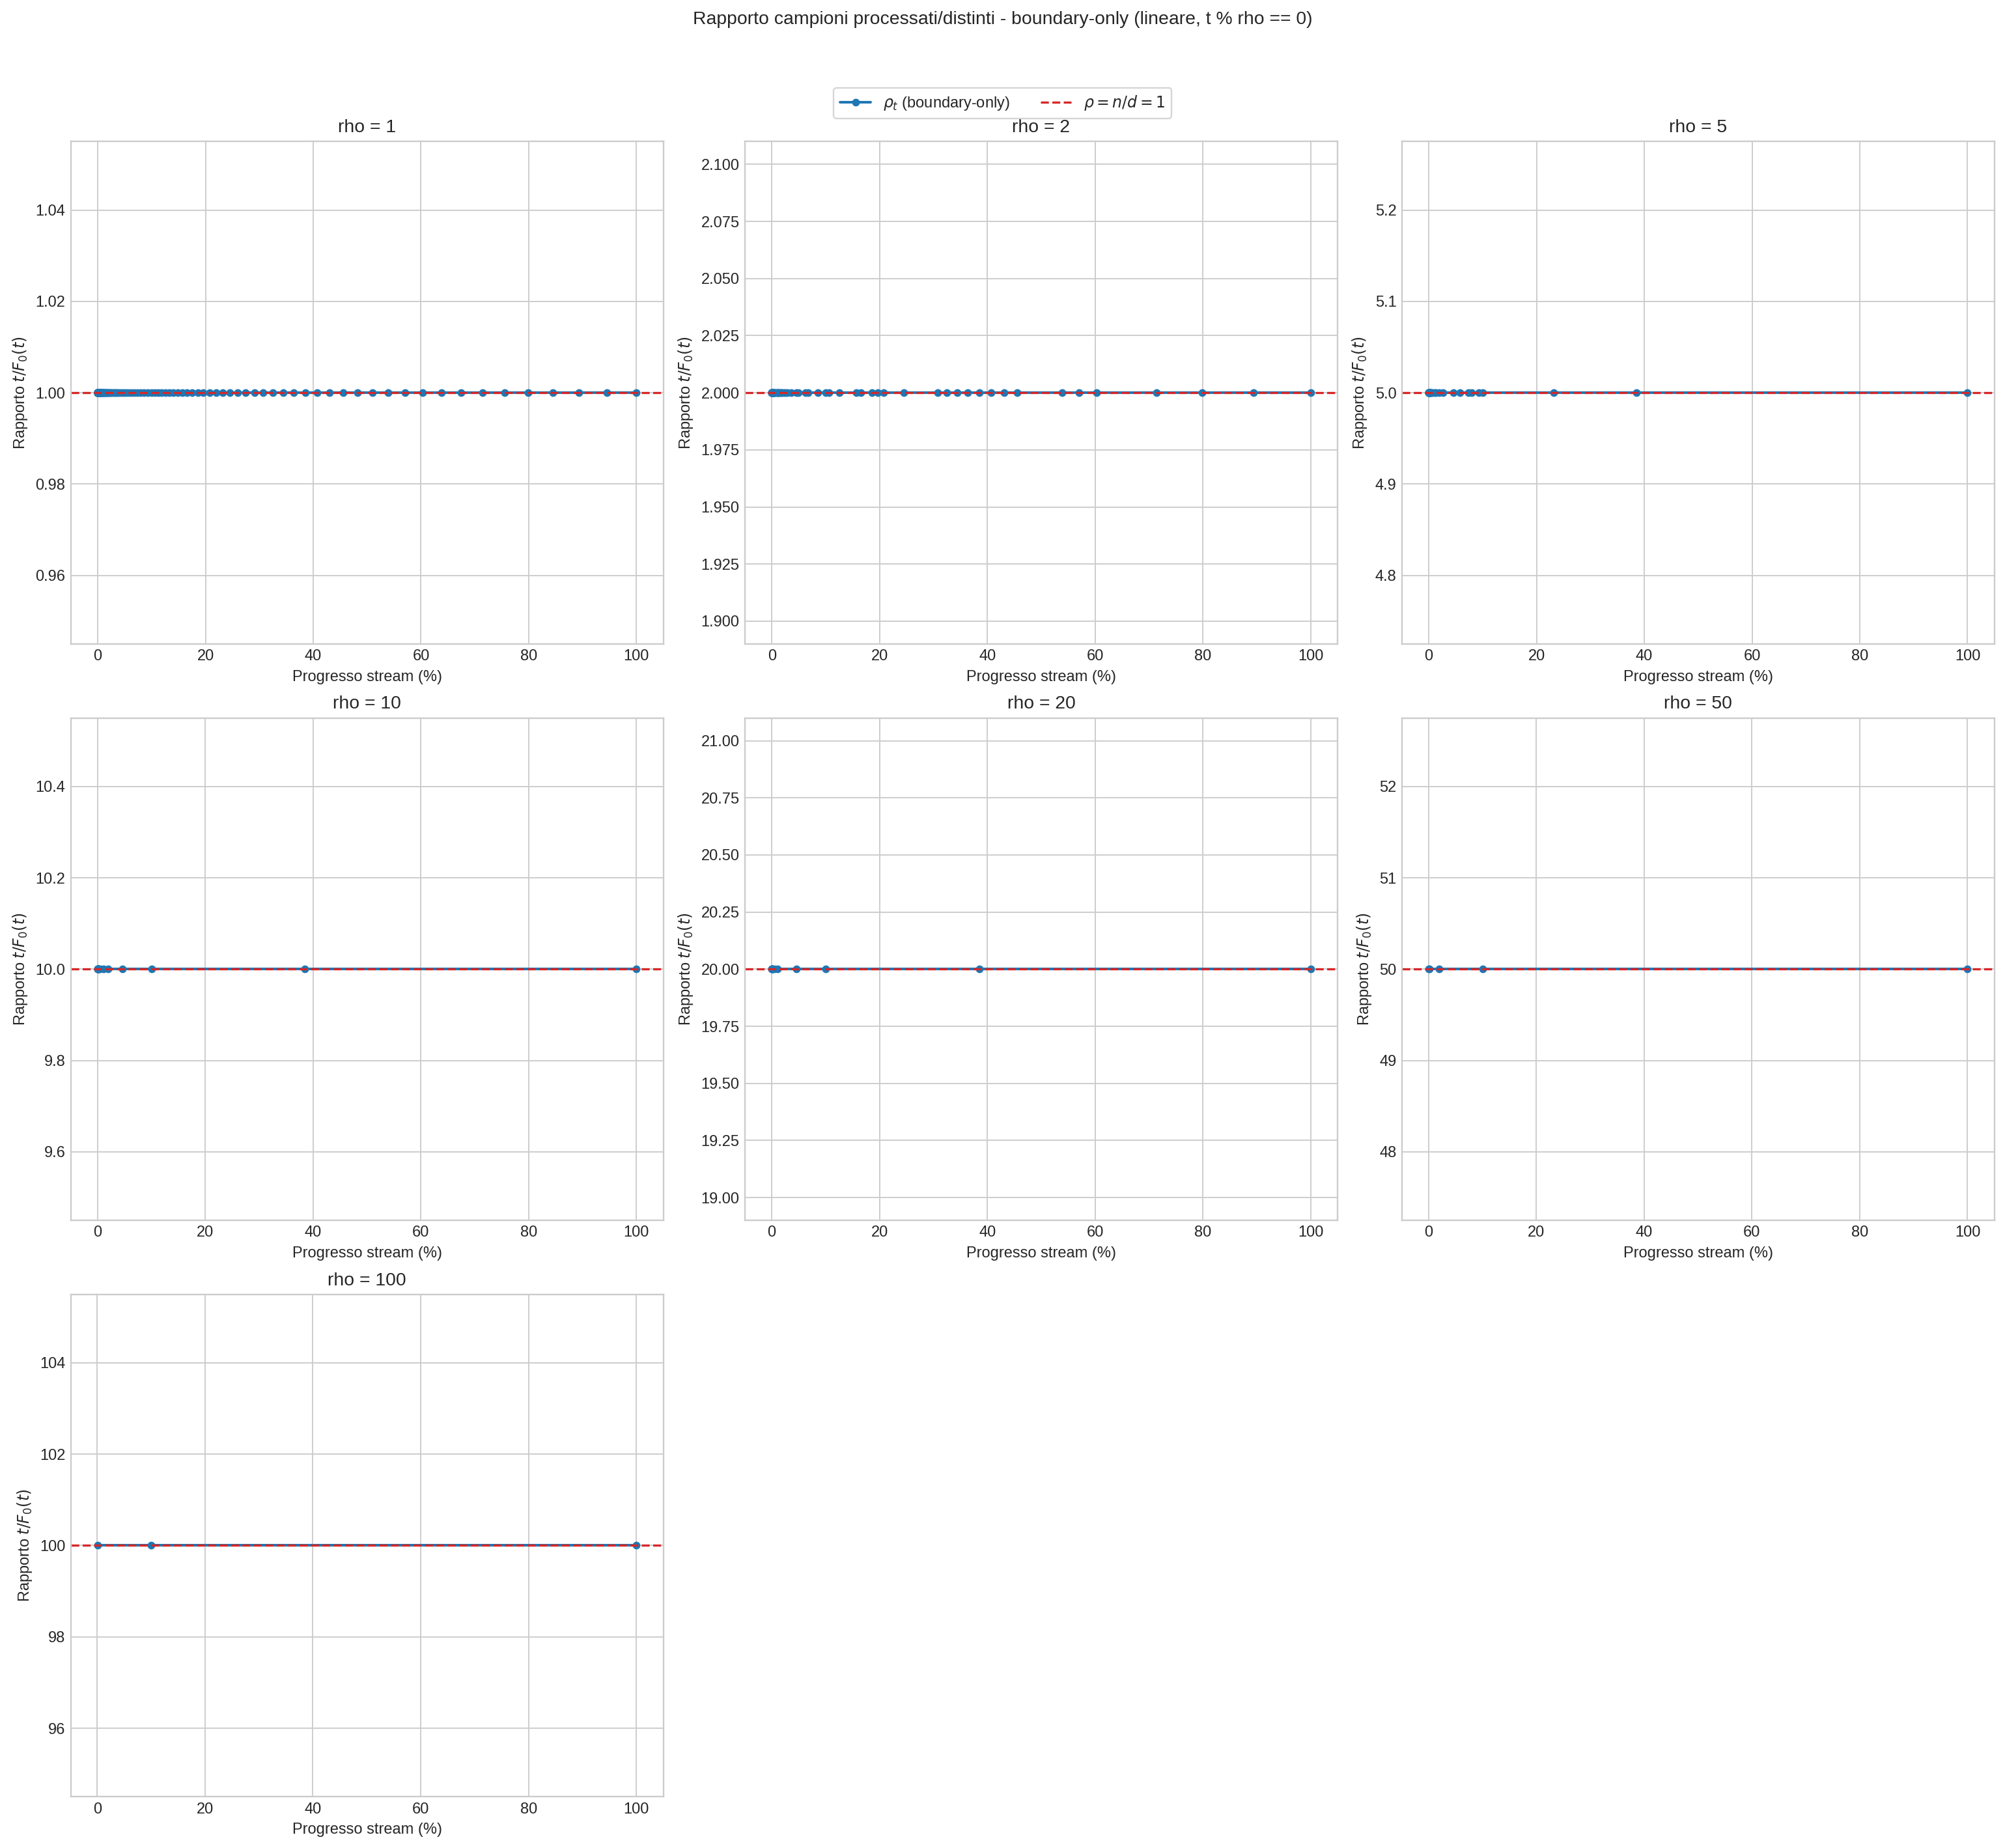
\includegraphics[width=0.96\textwidth]{figures/results/ratio_processed_vs_distinct_streaming_boundary_linear.png}
    \caption{Rapporto \(\rho_t\) osservato ai bordi di blocco}
    \label{fig:ch5-dataset-rho-ratio-boundary}
\end{figure}

\subsection{Scelta del seed}
Una verifica preliminare, svolta nelle prime iterazioni degli esperimenti, ha
indicato che l'effetto del seed resta ininfluente rispetto alle differenze tra
algoritmi e tra le varie modalit\`a di merge.

Non sono stati fatti confronti con pi\`u dataset con seed diversi ma stessi parametri
anche per una questione di spazio richiesto. 

Ogni dataset pesa nell'ordine dei 2 GB dopo la compressione, per 50 milioni di elementi.
Le configurazioni testate sono tante e sarebbe diventato arduo testarle tutte.

Per questo motivo gli esperimenti principali fissano un seed unico pari a
\(21041998\).

\section{Esperimenti sugli algoritmi}
Gli esperimenti sugli algoritmi sono organizzati in due gruppi complementari.
  Il primo ha lo scopo di osservare come cambia la qualità della stima al variare
  della cardinalità reale del prefisso e del rapporto tra elementi processati e
  distinti. L'interesse non è limitato al solo errore medio, ma comprende anche
  la dispersione della stima, così da distinguere chiaramente tra fenomeni di
  bias e fenomeni di scarsa robustezza.

  Per isolare questi effetti sono state considerate due viste del problema. Nella
  prima si fissa il rapporto
  \[
  \rho=\frac{n}{d}
  \]
  e si osserva la stima in funzione della cardinalità reale del prefisso. Nella
  seconda si fissano valori obiettivo della cardinalità reale e si studia la
  stima in funzione del rapporto medio di ripetizione del prefisso,
  \[
  \rho_t=\frac{t}{F_0(t)}
  \]
  in modo da separare, per quanto possibile, l'effetto della crescita dei distinti
  da quello delle ripetizioni medie.

  Il secondo gruppo di esperimenti mantiene fisso il contesto di esecuzione e
  varia invece il parametro interno di precisione di ciascun algoritmo. Questa
  analisi serve a capire non solo quale algoritmo sia più accurato nel complesso,
  ma anche quanto il suo comportamento dipenda dalla scelta del parametro e se il
  miglioramento ottenuto all'aumentare delle risorse sia regolare oppure no.
\subsection{Configurazione utilizzata}

Gli esperimenti usano il dataset:
\begin{center}
\small
\codepath{datasets/prefix_constant_rho/dataset_n_10000000_d_<d>_p_50_s_21041998.bin}
\end{center}

I risultati sono salvati in:
\begin{center}
\small
\codepath{results/prefix_constant_rho/streaming/.../results_streaming.csv}
\end{center}

Le metriche principali osservate sono:
\begin{itemize}
    \item cardinalità reale del prefisso \(\,F_0(t)\,\) in
    \texttt{f0\_mean\_t};
    \item stima media \(\,\hat{F}_0(t)\,\) in \texttt{f0\_hat\_mean\_t};
    \item dispersione della stima con bande \(\mu \pm \sigma\);
    \item errore relativo medio ai punti finali osservati, usato come sintesi
    comparativa tra algoritmi.
\end{itemize}

\subsection{Analisi della robustezza degli algoritmi}
L'obiettivo di questa parte è capire rispetto a quali parametri gli algoritmi si
  comportino bene o male. I due parametri considerati sono il numero reale di
  elementi distinti osservati in un prefisso e il rapporto tra elementi processati
  e distinti, cioè il numero medio di ripetizioni del prefisso.

  L'analisi tiene conto di due aspetti diversi della qualità della stima. Il primo
  è il bias, cioè lo scostamento sistematico tra il valore medio stimato e il
  numero corretto di elementi distinti. Il secondo è la robustezza, cioè la
  dispersione della stima attorno al suo valore medio: uno stimatore può anche
  essere corretto in media, ma restare comunque molto sensibile al rumore e quindi
  presentare una varianza elevata. Per questa ragione, nei grafici vengono
  mostrati insieme il valore medio della stima e la sua dispersione.

  Per studiare separatamente la dipendenza da questi due parametri, sono stati
  adottati due protocolli sperimentali distinti.

  Nel primo caso, chiamato per facilit\`a caso $A$, si fissa il rapporto
  \[
  \rho=\frac{n}{d}
  \]
  e si osserva l'andamento della stima al variare del numero reale di elementi
  distinti presenti nel prefisso. In questo modo si analizza come cambino bias e
  dispersione a parità di ripetizione media.

  Nel secondo caso, chiamato caso $B$, si fissano alcuni valori target della cardinalità reale e si
  osserva la stima in funzione del rapporto medio di ripetizione del prefisso,
  calcolato come
  \[
  \rho_t=\frac{t}{F_0(t)}
  \]
  Questa scelta è necessaria perché usare il numero grezzo di elementi processati
  come ascissa introdurrebbe implicitamente anche una dipendenza dal numero di
  elementi distinti. Il rapporto \(\rho_t\) permette invece di isolare meglio
  l'effetto delle ripetizioni medie sul comportamento degli algoritmi.
\subsubsection{Stima in funzione della cardinalità reale del prefisso}
\label{sec:ch5-streaming-f0}

Questa analisi corrisponde ai grafici precedentemente indicati come
analisi del caso A.
L'ascissa riporta la cardinalità reale \(F_0(t)\), l'ordinata la stima
\(\hat{F}_0(t)\), e i pannelli sono separati per ciascun valore di \(\rho\).

\begin{figure}[p]
    \centering
    \begin{subfigure}[t]{0.49\textwidth}
        \centering
        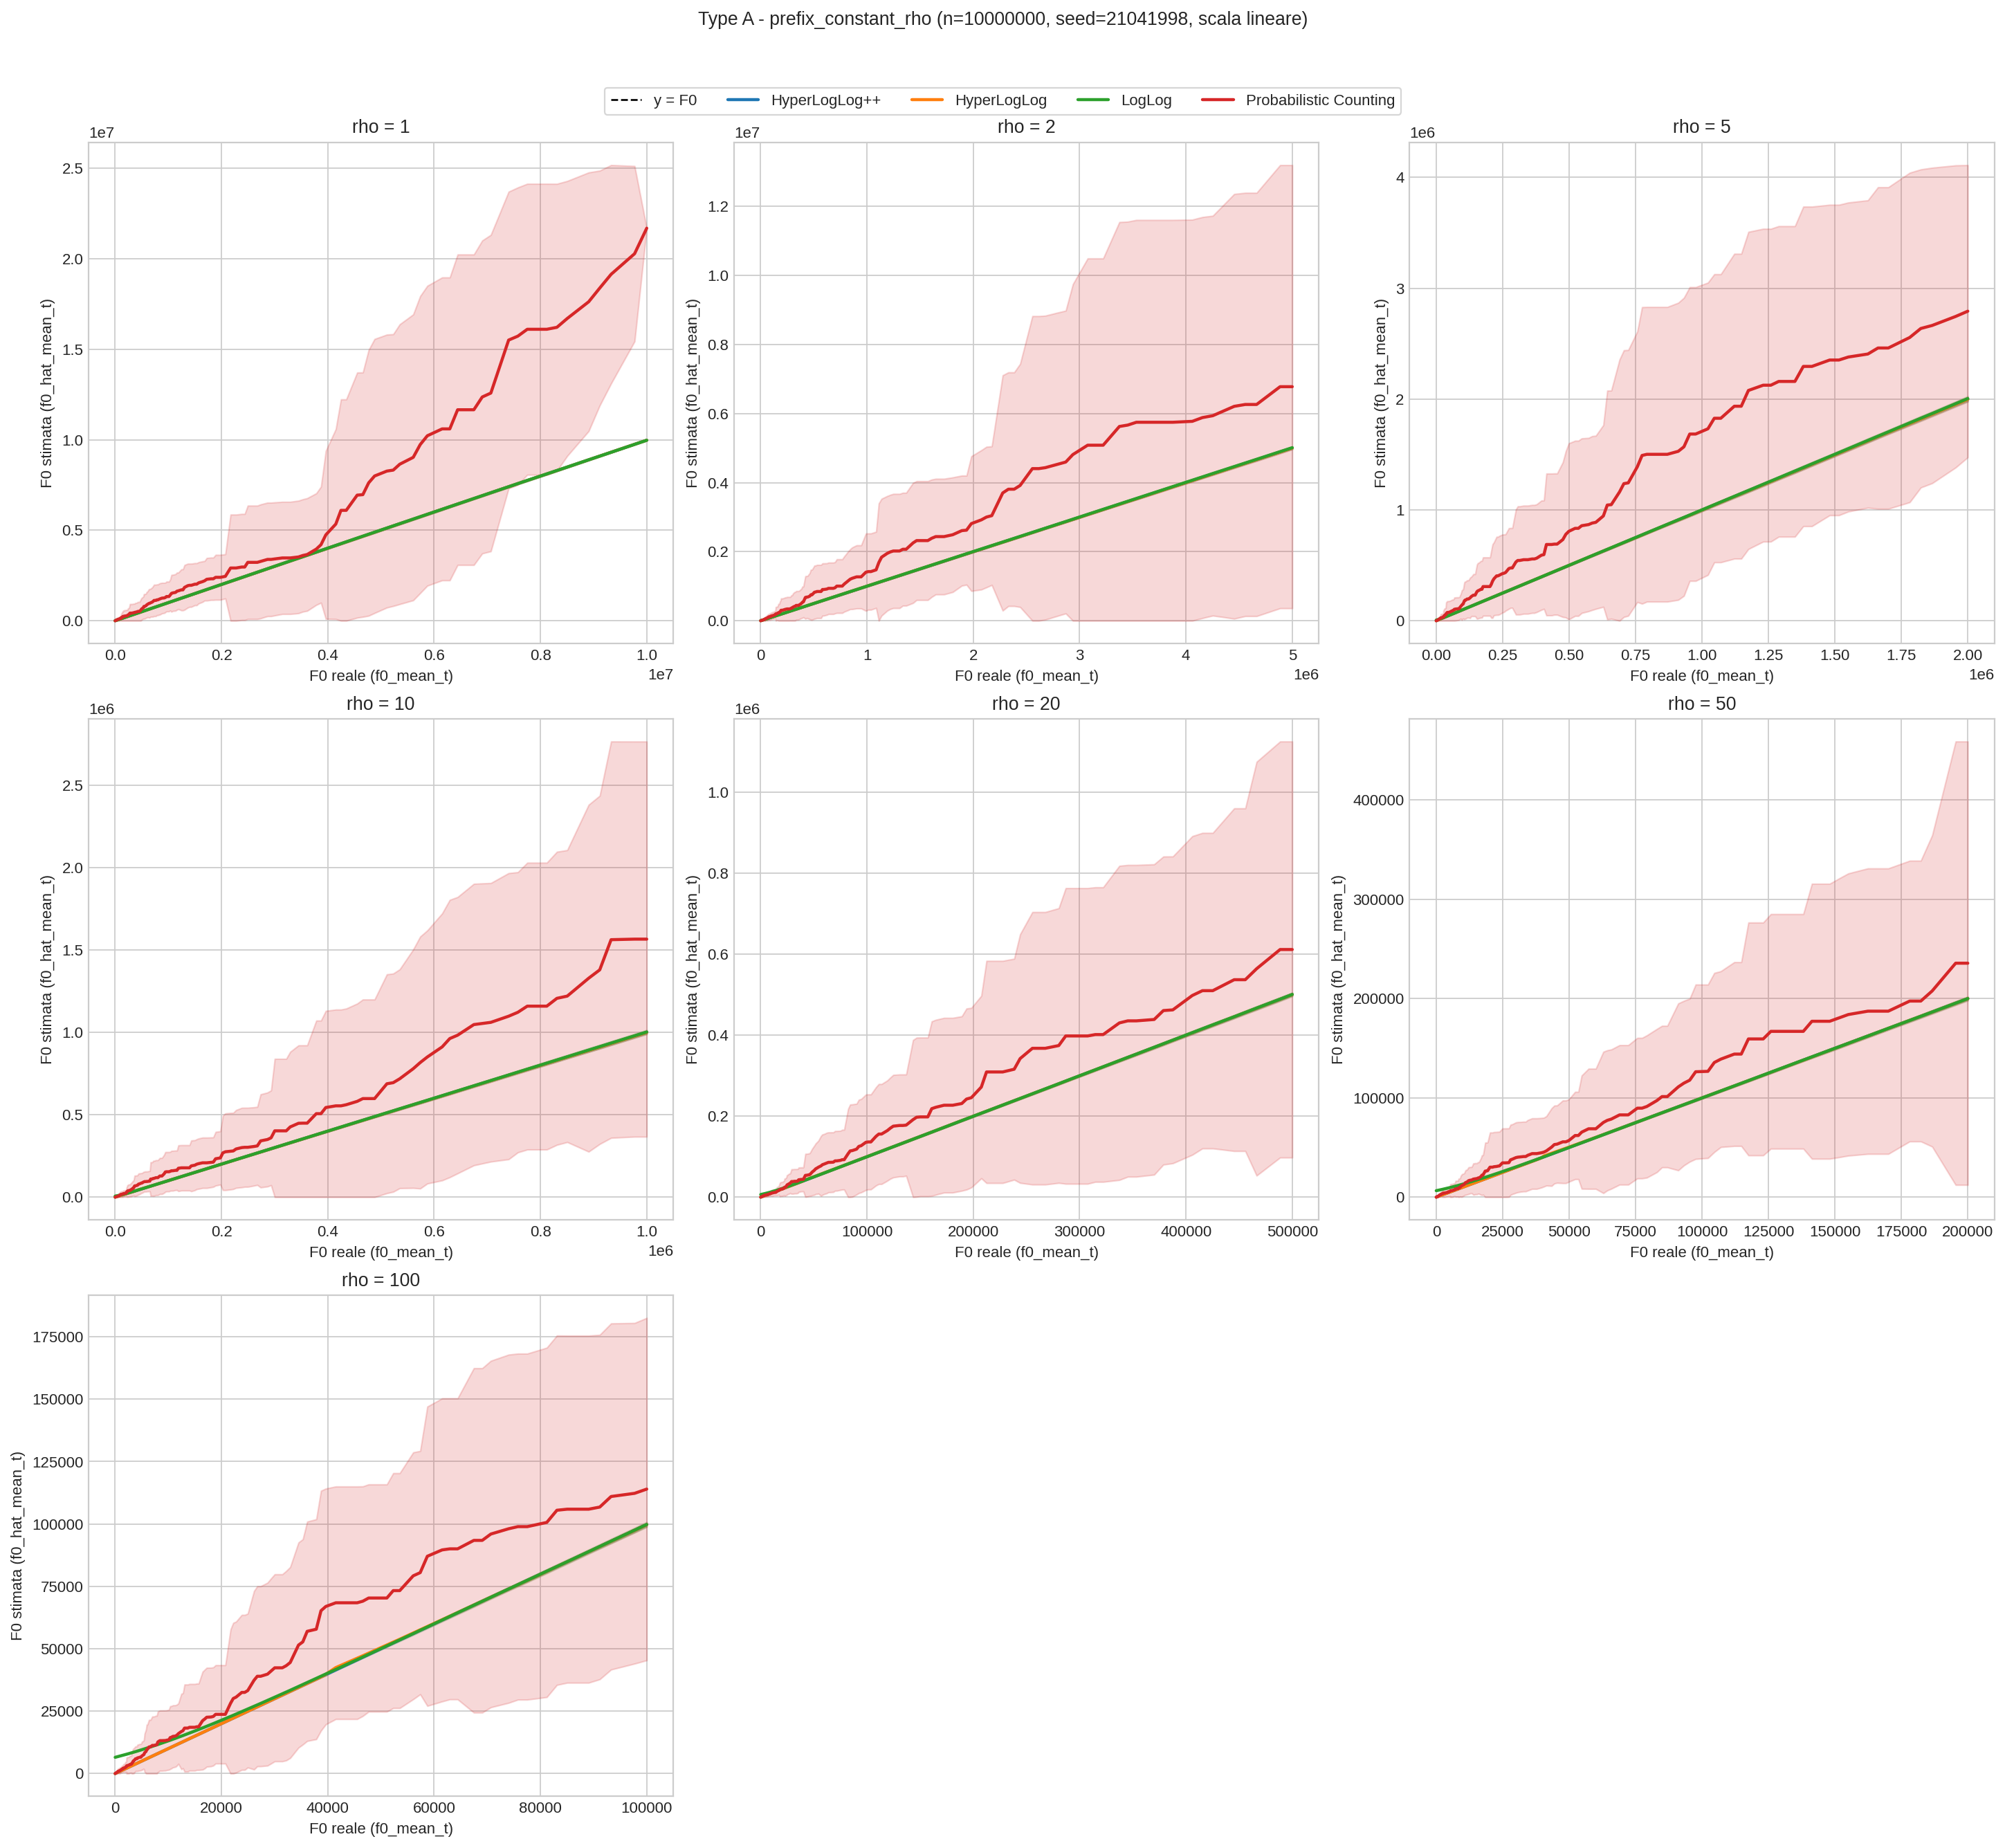
\includegraphics[width=\linewidth]{figures/results/typeA_prefix_constant_rho_linear.png}
        \caption{Scala lineare}
        \label{fig:ch5-stream-f0-all-linear}
    \end{subfigure}
    \hfill
    \begin{subfigure}[t]{0.49\textwidth}
        \centering
        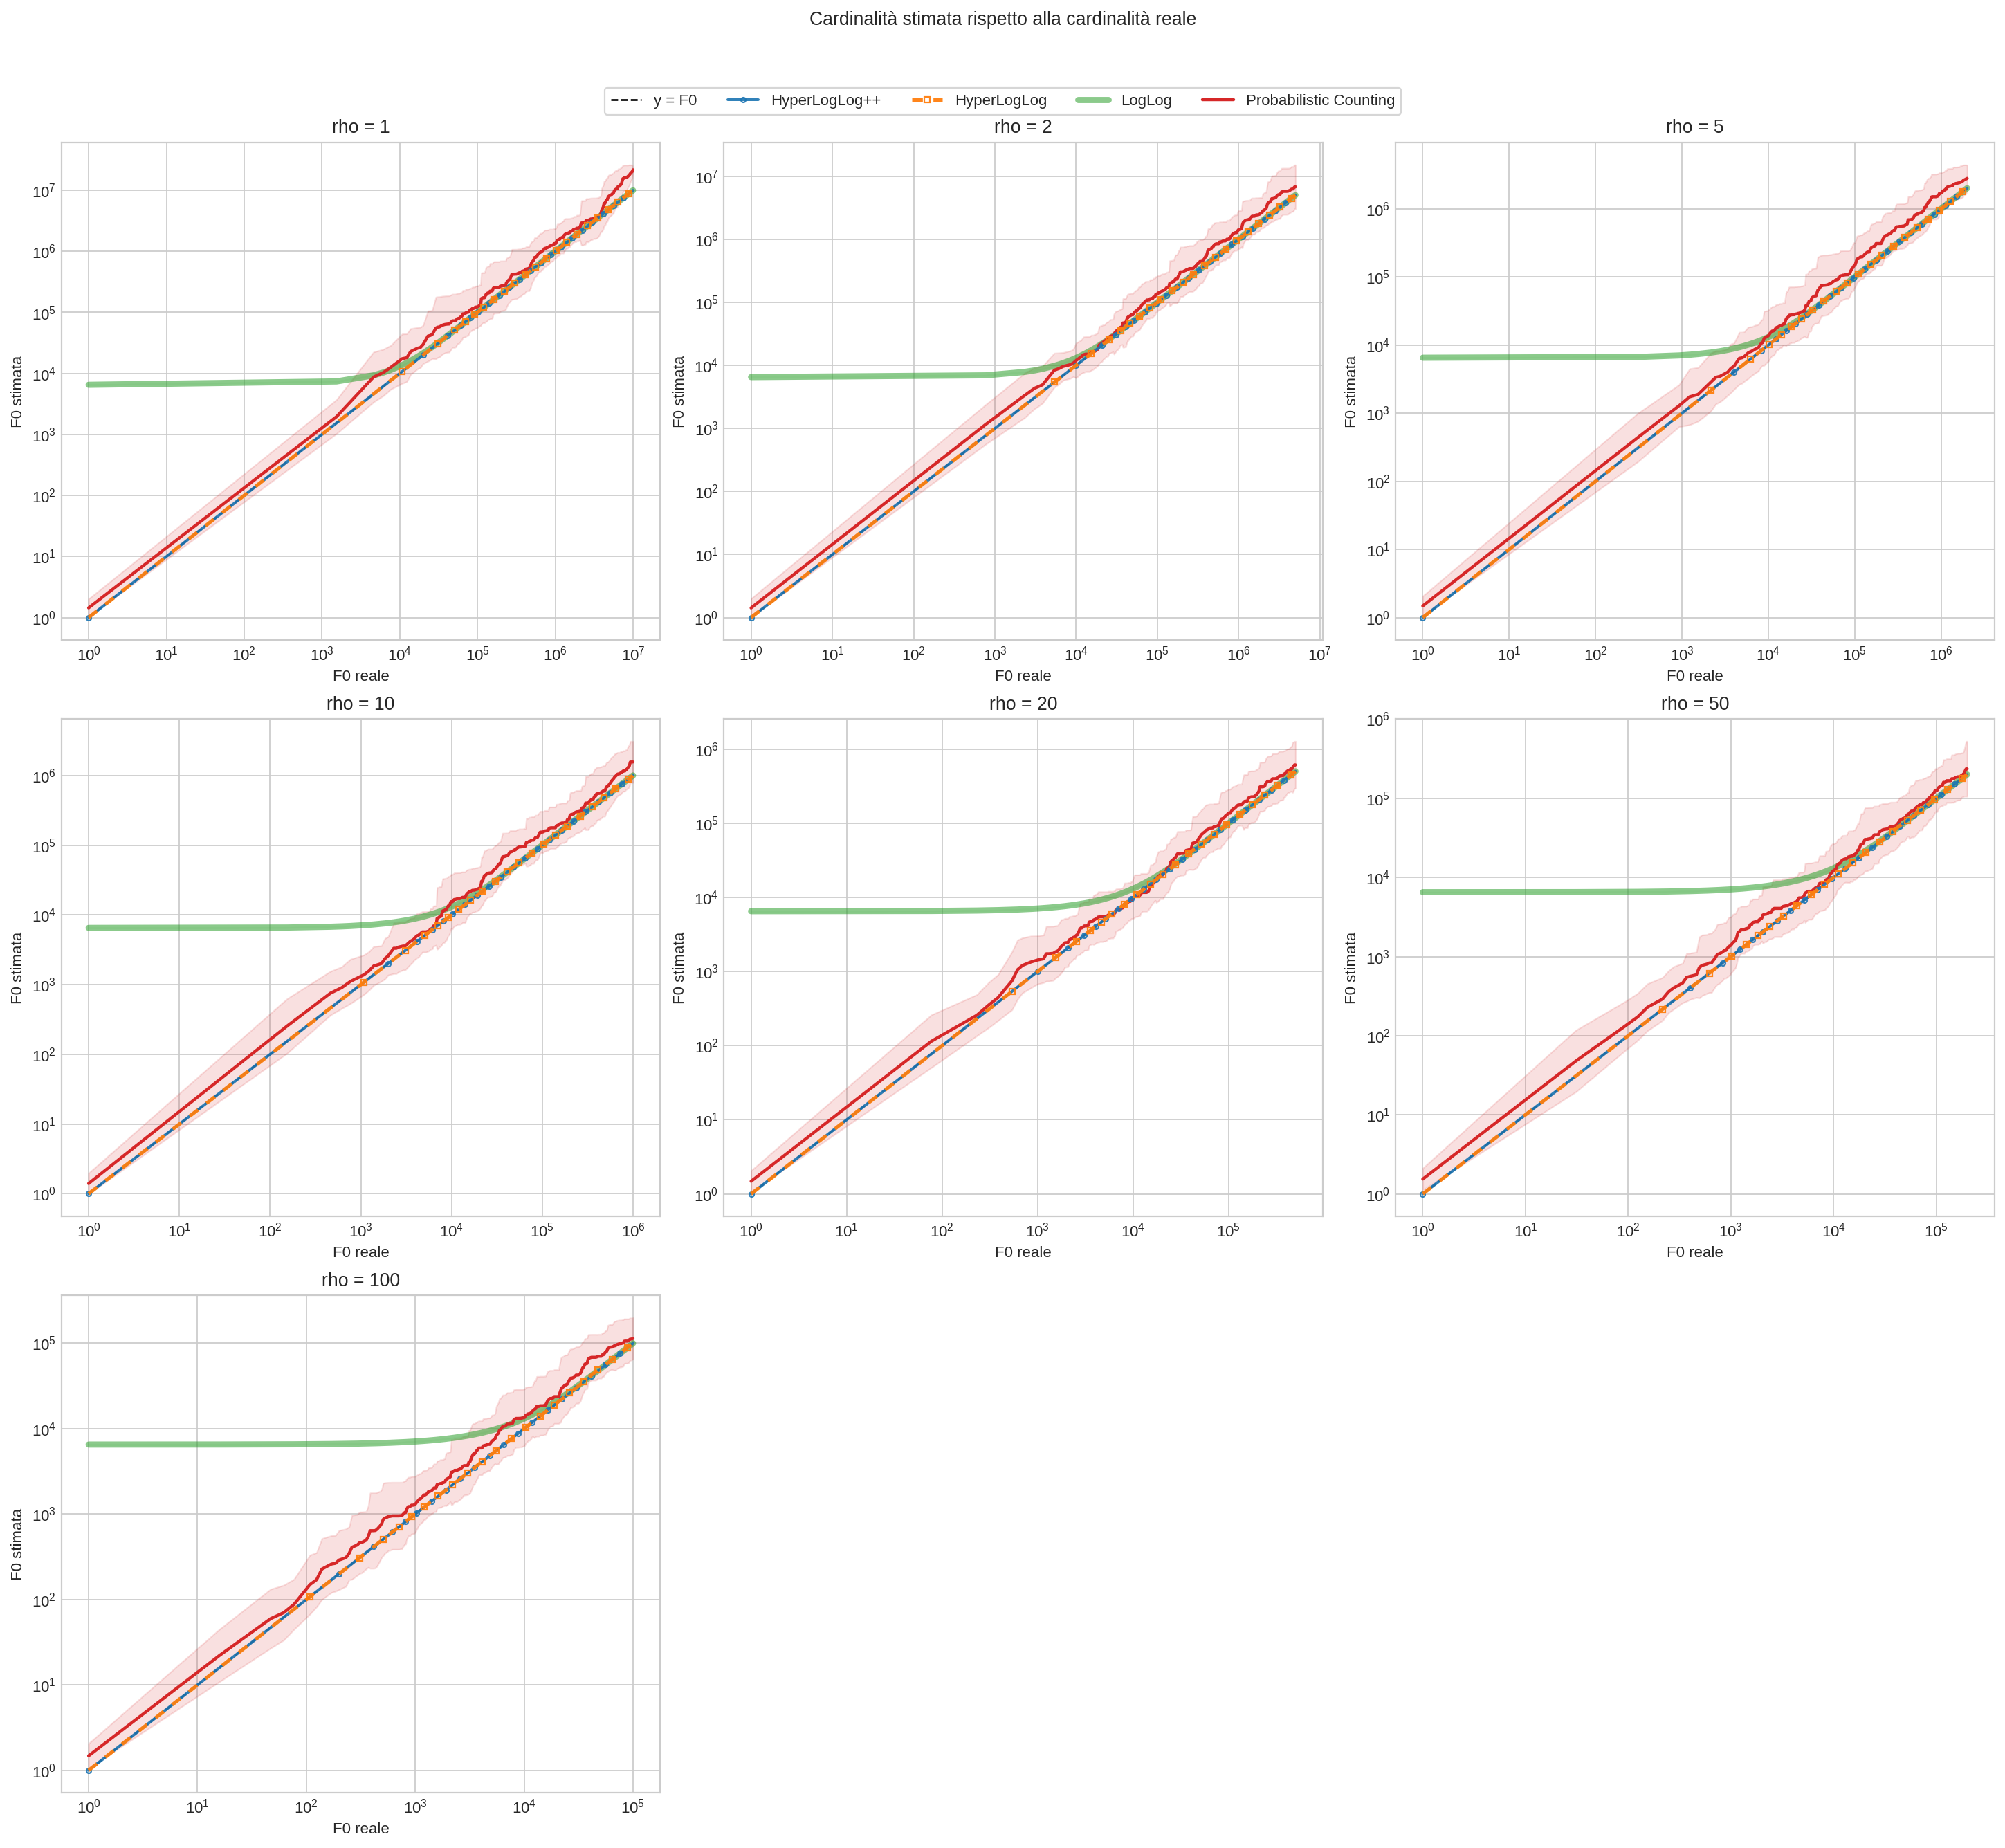
\includegraphics[width=\linewidth]{figures/results/typeA_prefix_constant_rho_loglog.png}
        \caption{Scala logaritmica}
        \label{fig:ch5-stream-f0-all-loglog}
    \end{subfigure}
    \caption{Stima rispetto alla cardinalità reale del prefisso, tutti gli algoritmi}
    \label{fig:ch5-stream-f0-all}
\end{figure}

\begin{figure}[p]
    \centering
    \begin{subfigure}[t]{0.49\textwidth}
        \centering
        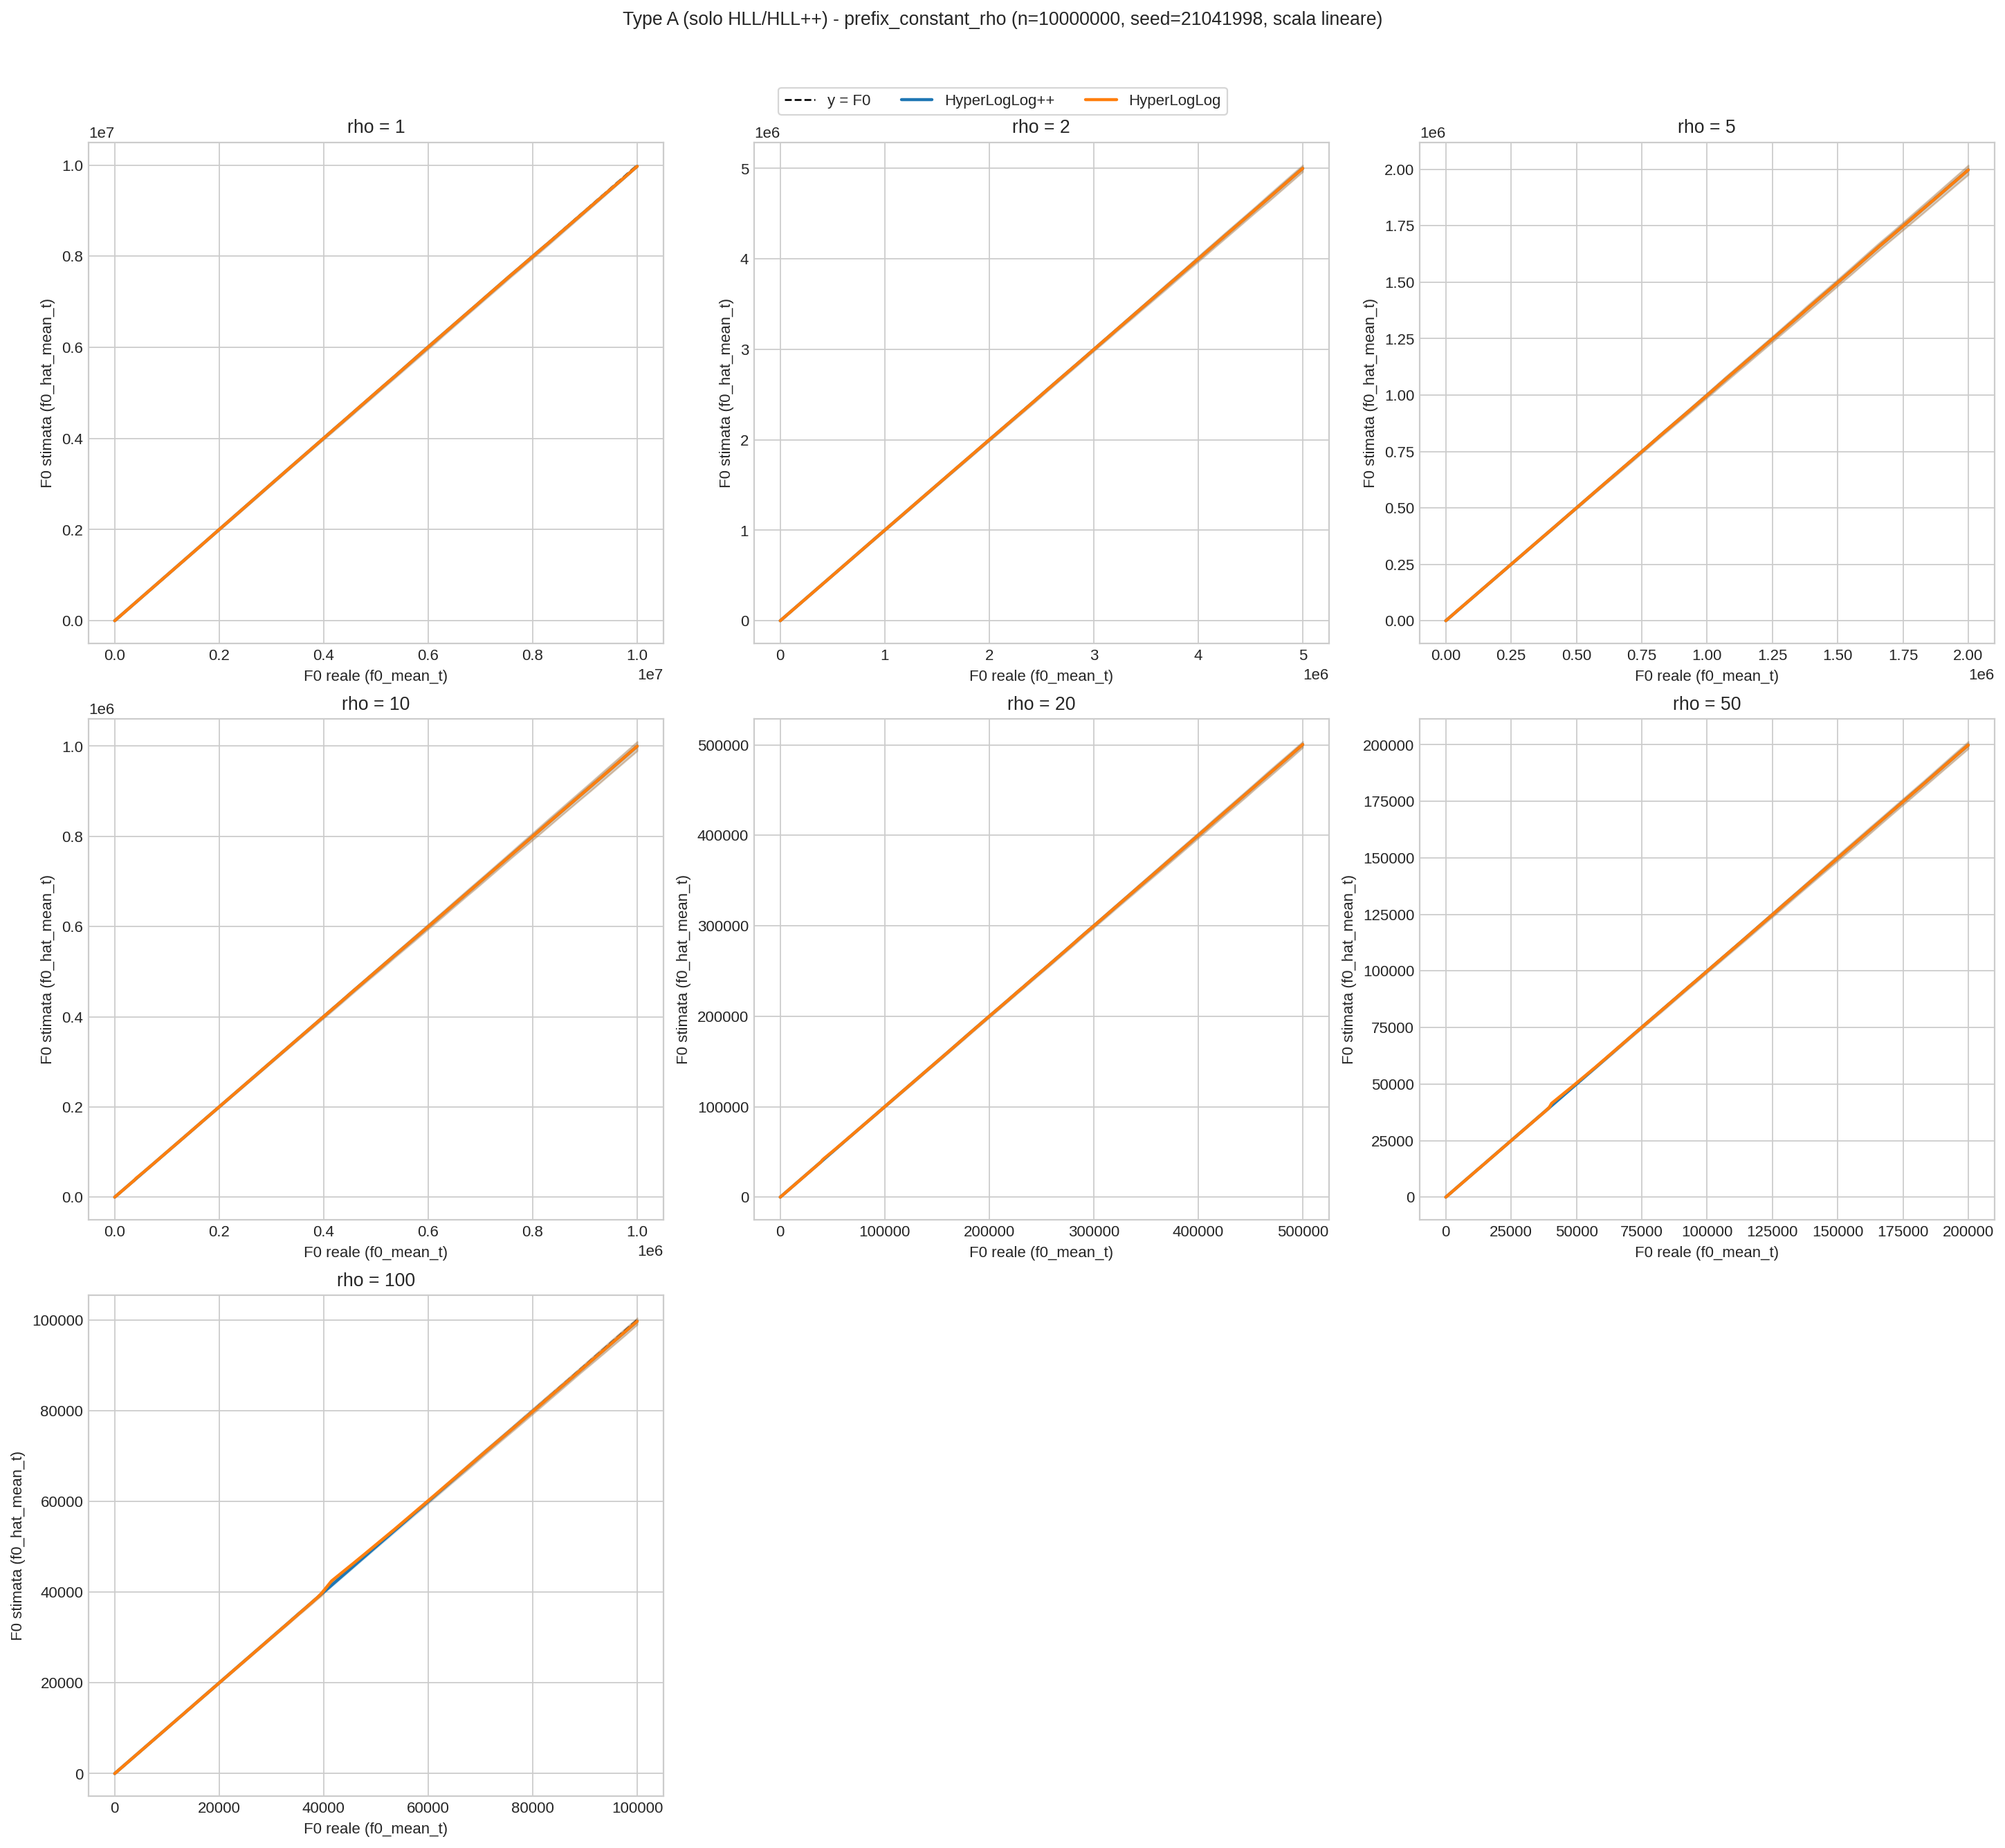
\includegraphics[width=\linewidth]{figures/results/typeA_prefix_constant_rho_hll_hllpp_linear.png}
        \caption{Scala lineare}
        \label{fig:ch5-stream-f0-hll-linear}
    \end{subfigure}
    \hfill
    \begin{subfigure}[t]{0.49\textwidth}
        \centering
        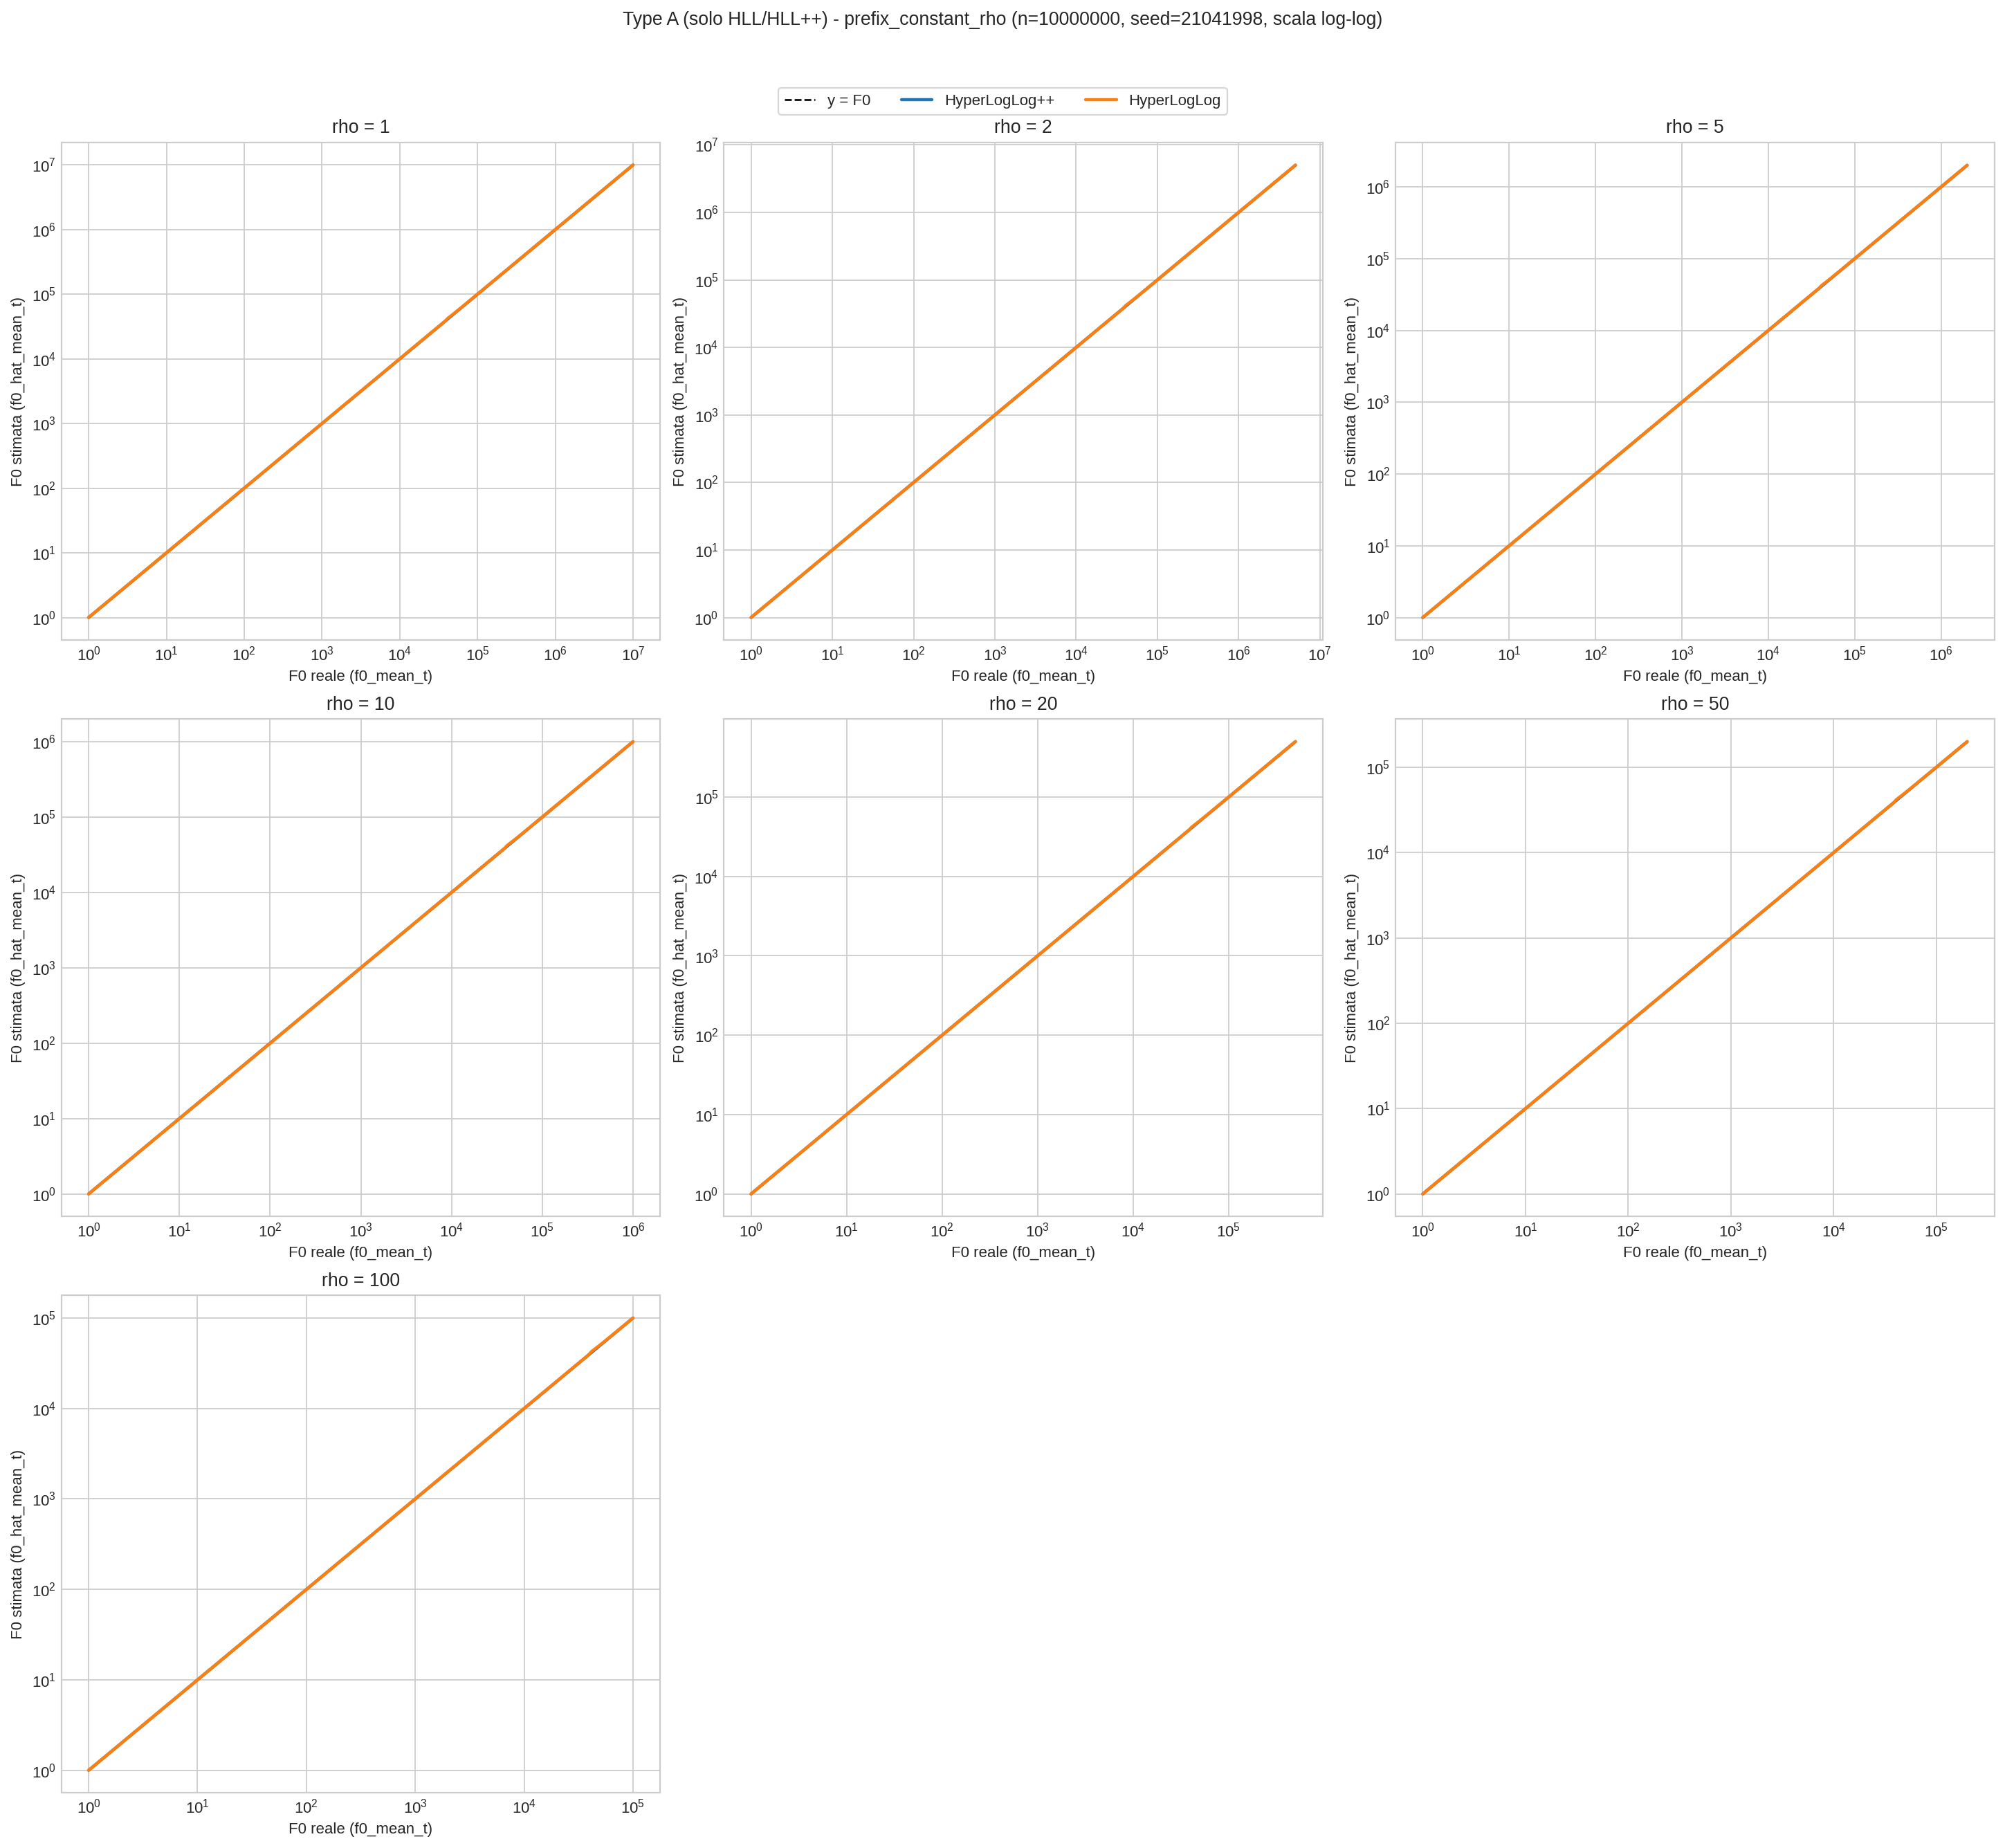
\includegraphics[width=\linewidth]{figures/results/typeA_prefix_constant_rho_hll_hllpp_loglog.png}
        \caption{Scala logaritmica}
        \label{fig:ch5-stream-f0-hll-loglog}
    \end{subfigure}
    \caption{Stima rispetto alla cardinalità reale del prefisso, confronto HyperLogLog e HyperLogLog++}
    \label{fig:ch5-stream-f0-hll}
\end{figure}

\subsubsection{Stima in funzione del rapporto tra elementi processati e distinti}
\label{sec:ch5-streaming-rho}

Questa analisi corrisponde ai grafici precedentemente indicati come
analisi del caso B.
Per ciascun valore obiettivo
\[
F_0^{\ast} \in \{1000,2000,5000,10000,20000,50000,100000\}
\]
si estrae per interpolazione il punto la cui ascissa è il rapporto
\[
\rho_t=\frac{t}{F_0(t)}
\]
e la cui ordinata è la stima corrispondente.

\begin{figure}[p]
    \centering
    \begin{subfigure}[t]{0.49\textwidth}
        \centering
        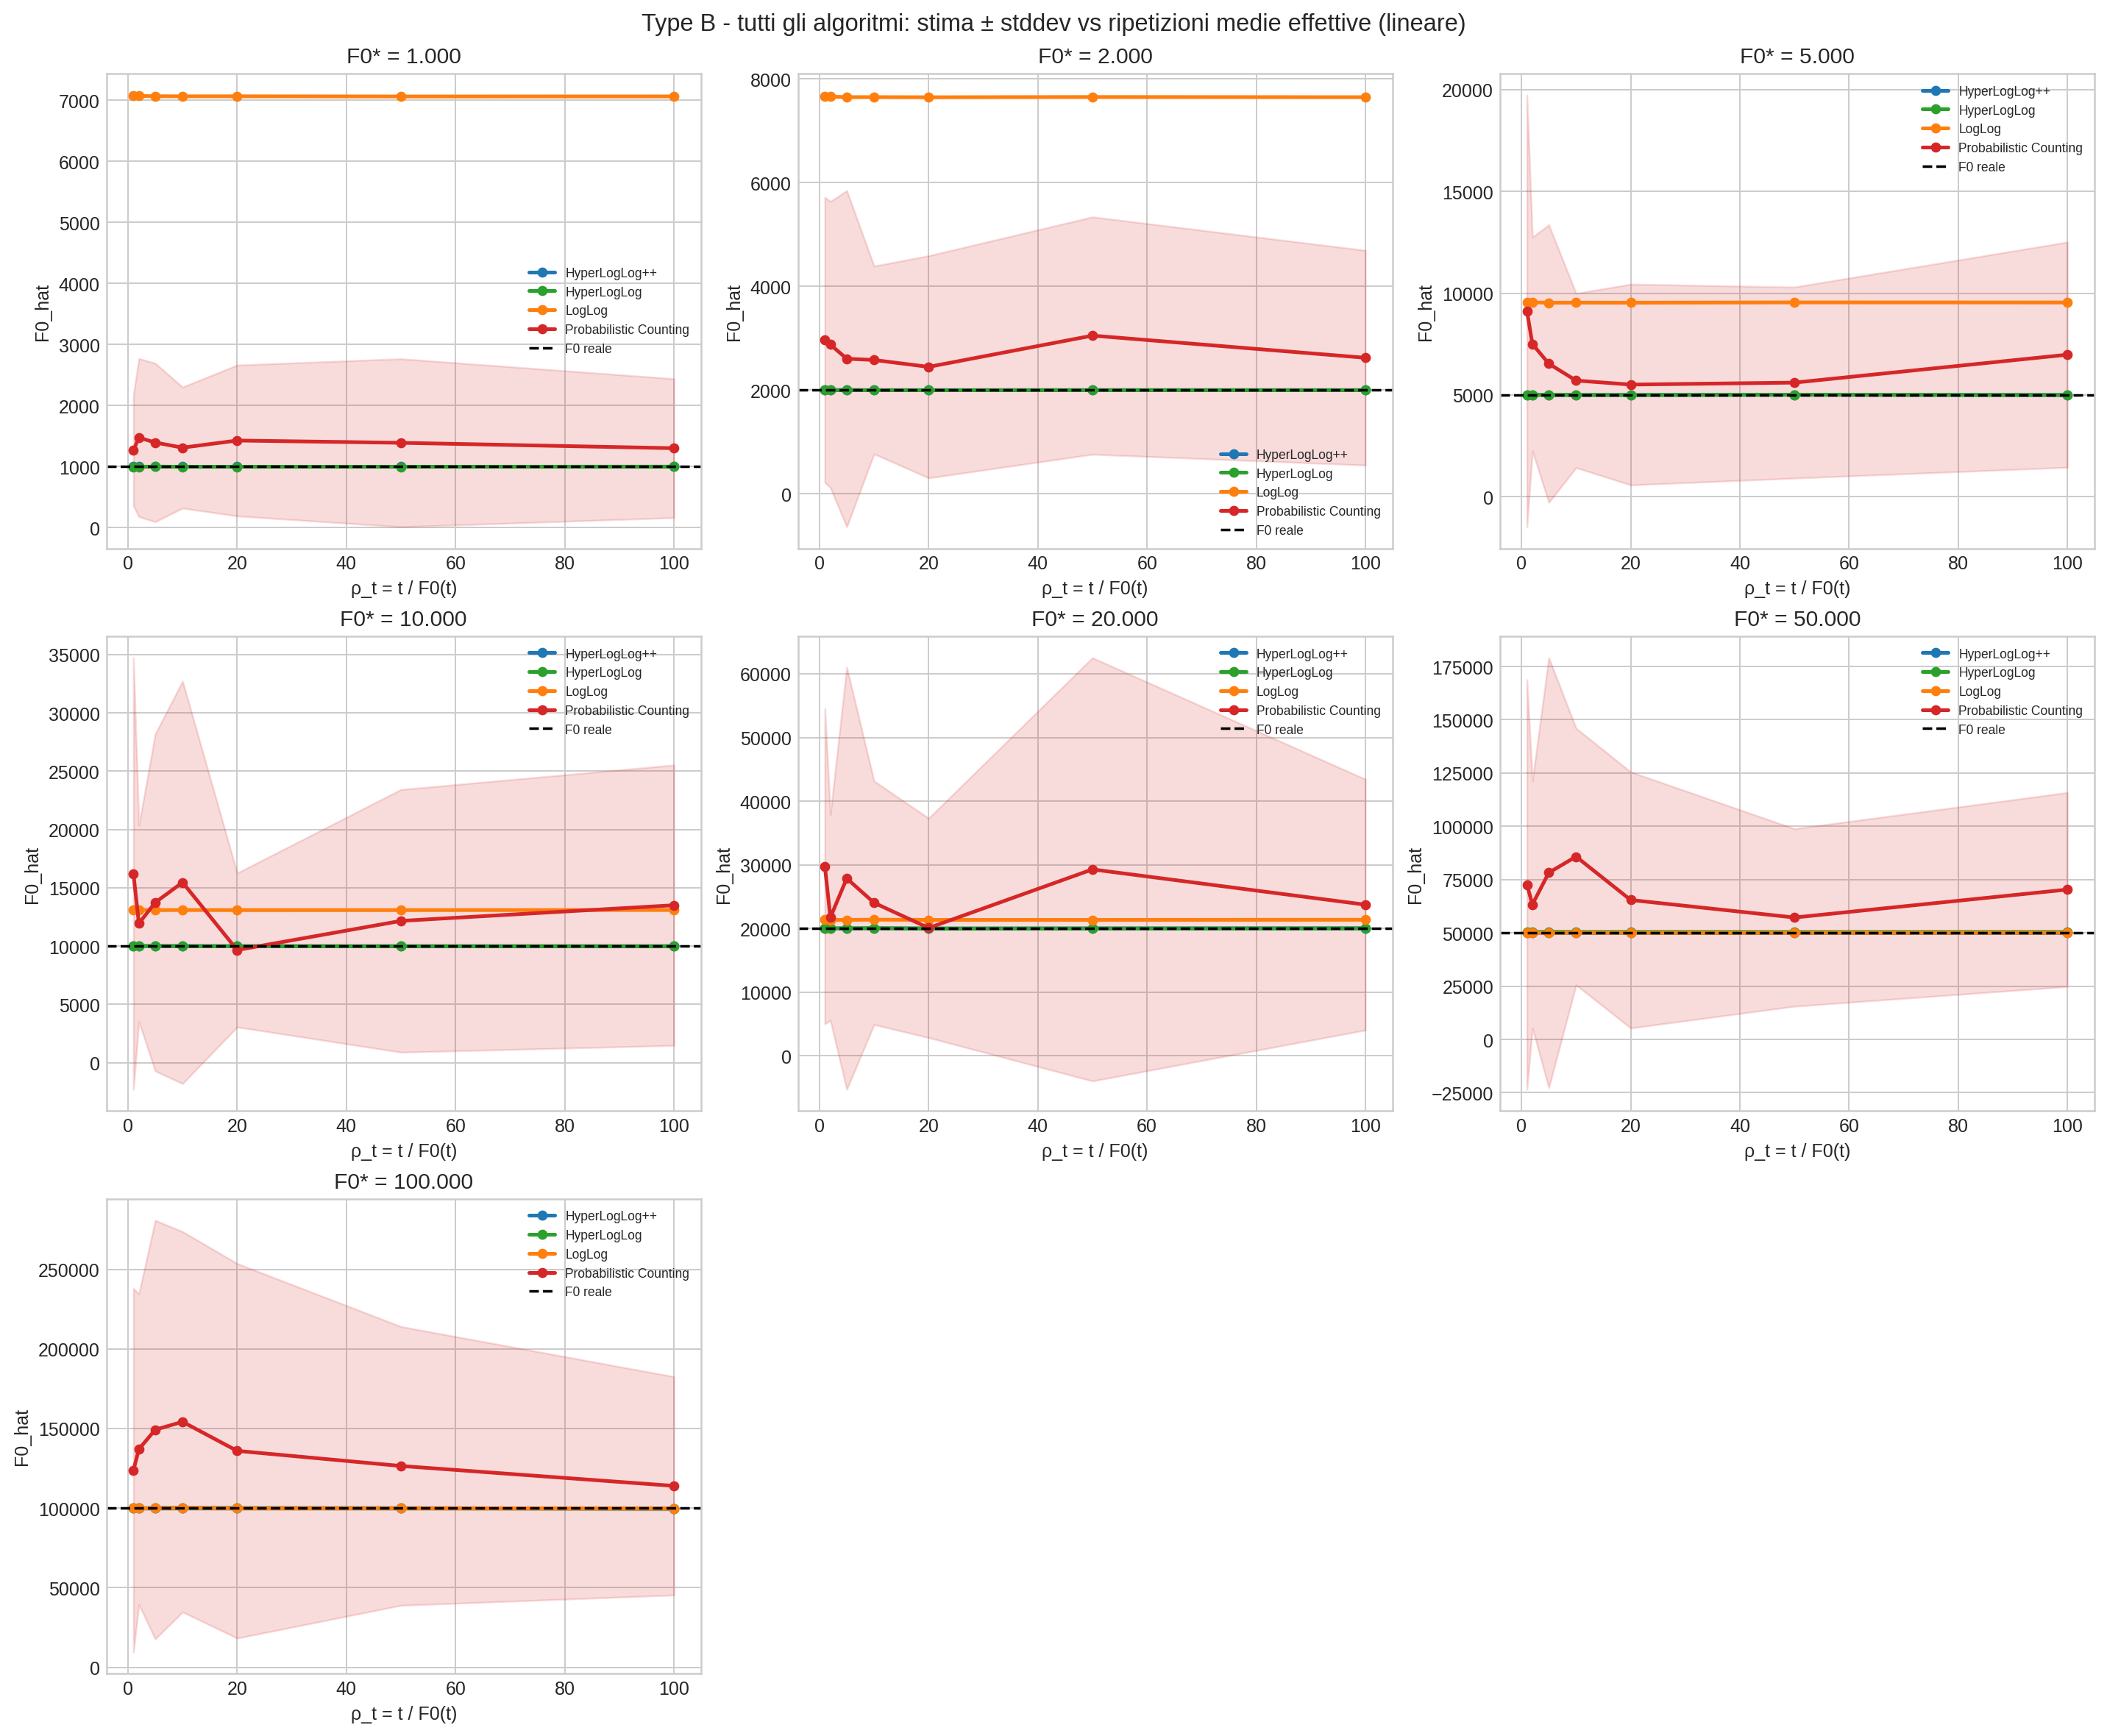
\includegraphics[width=\linewidth]{figures/results/typeB_prefix_constant_rho_all_linear.png}
        \caption{Scala lineare}
        \label{fig:ch5-stream-rho-all-linear}
    \end{subfigure}
    \hfill
    \begin{subfigure}[t]{0.49\textwidth}
        \centering
        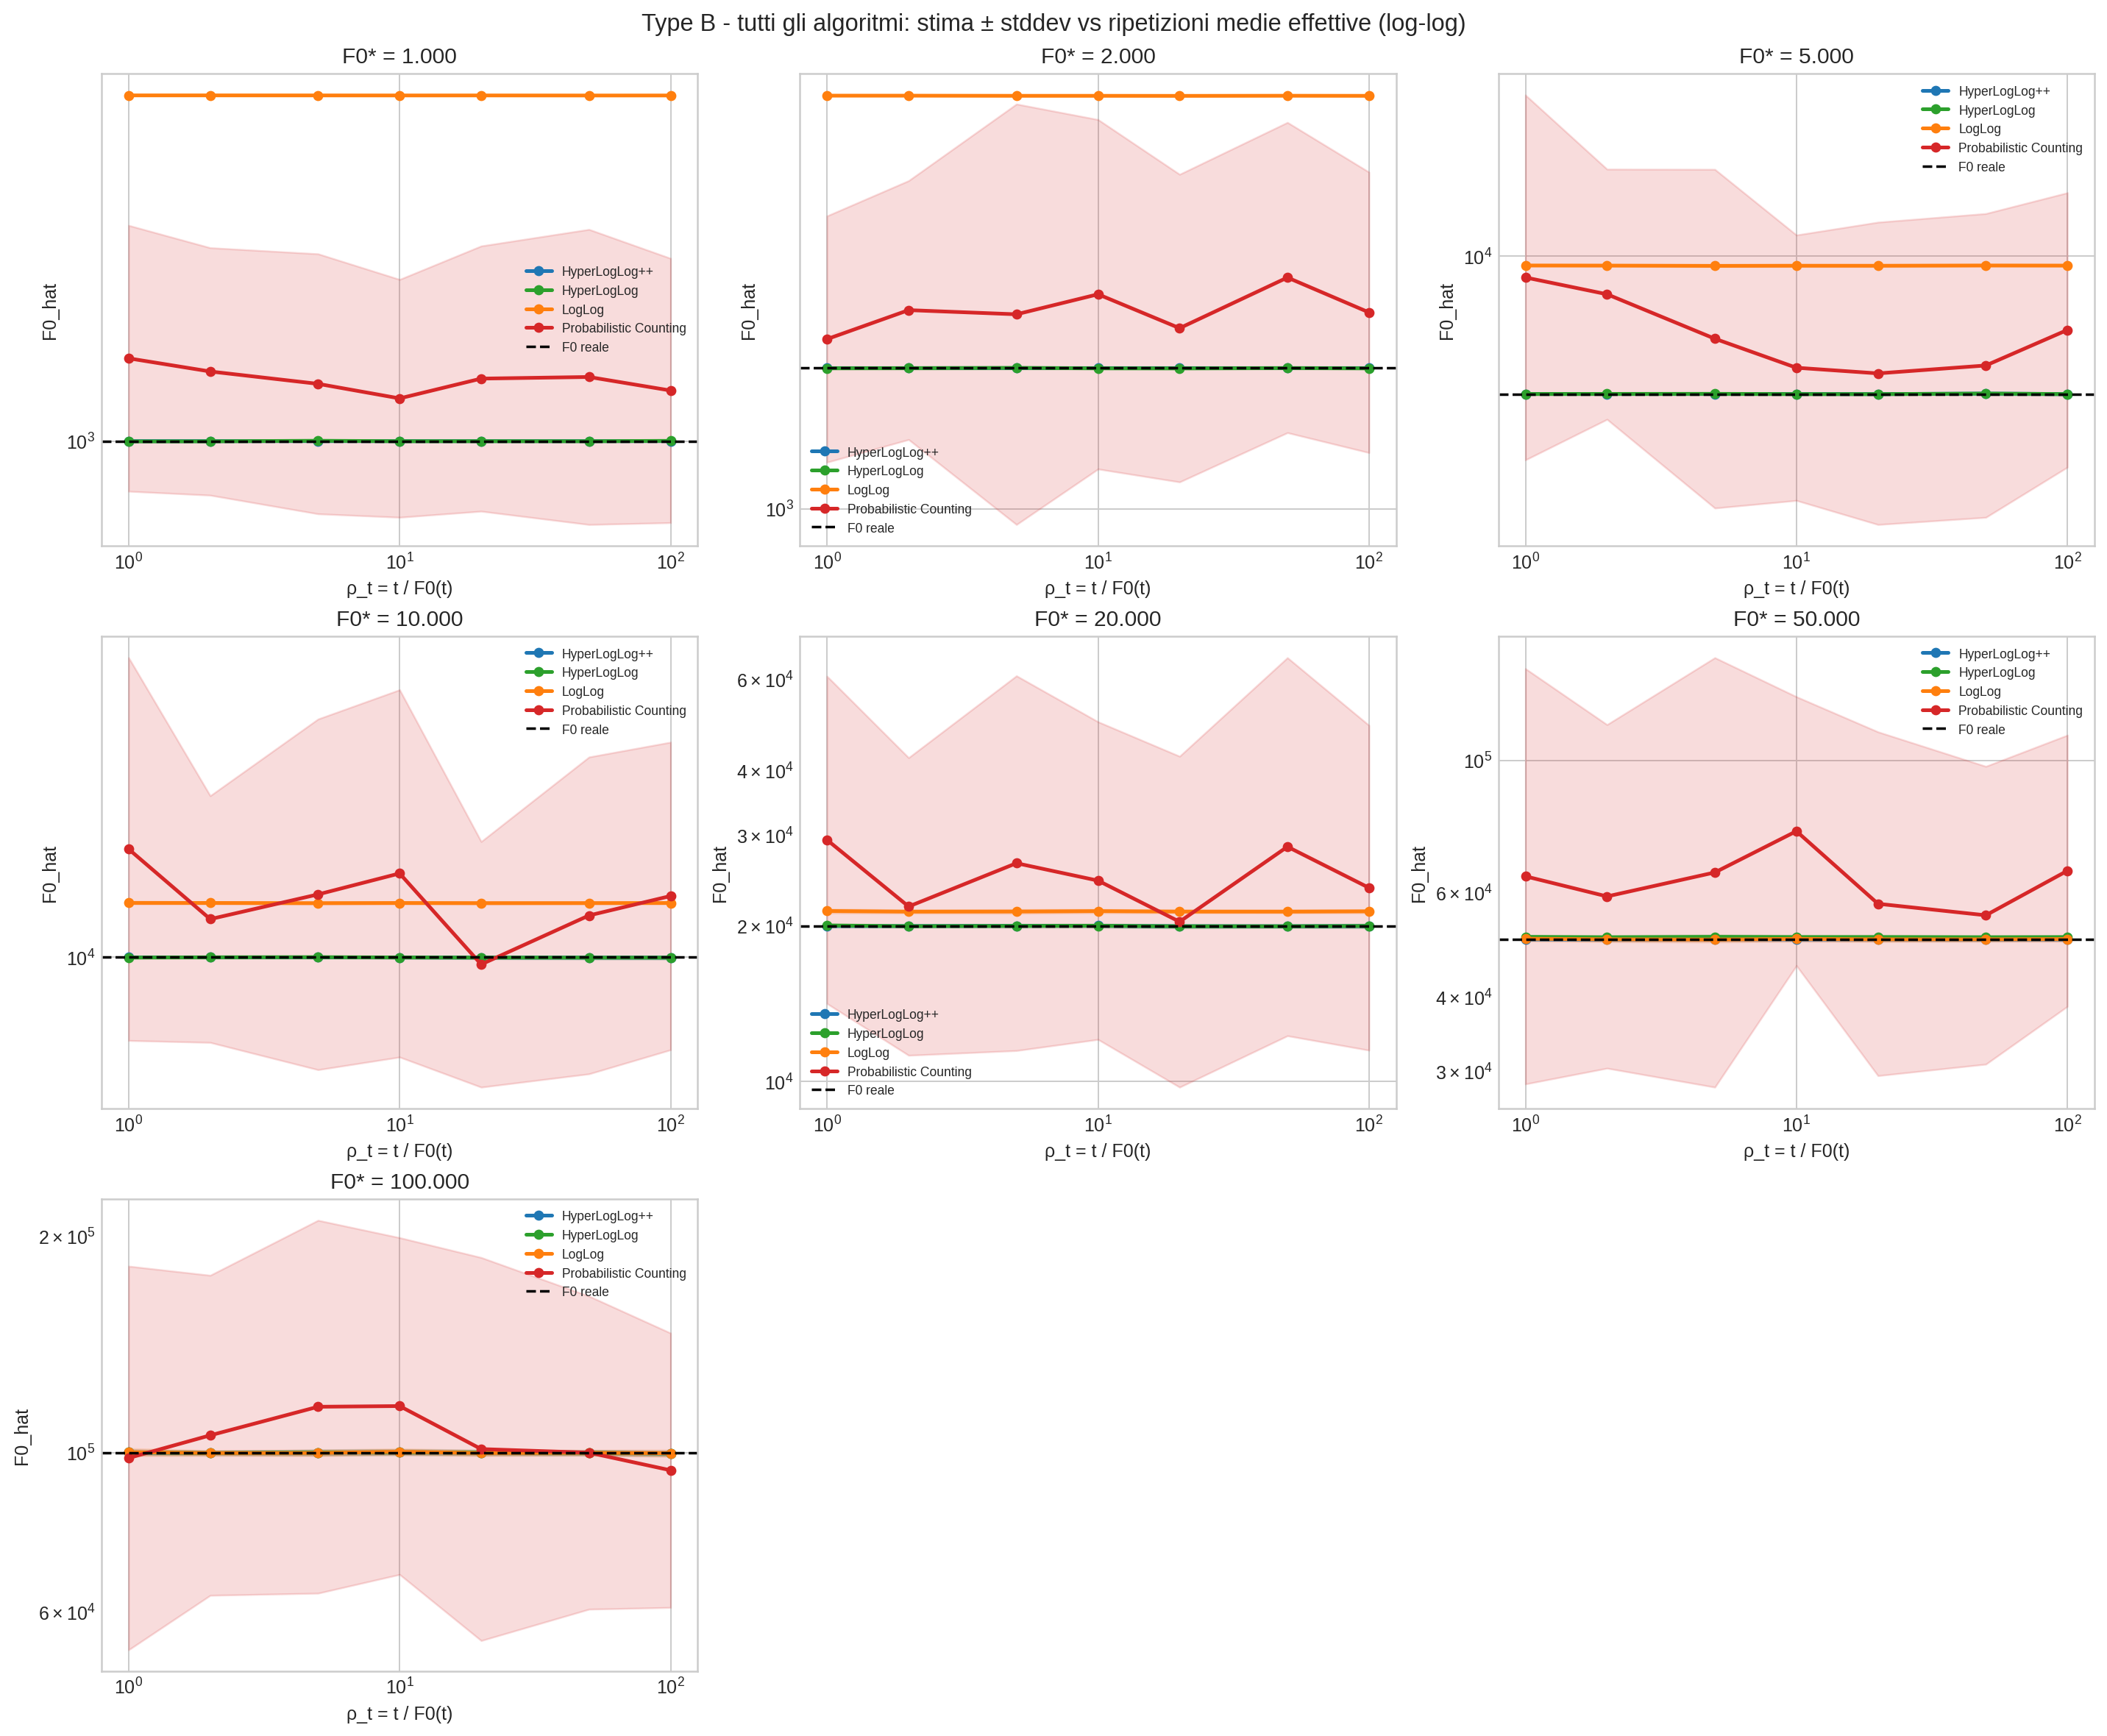
\includegraphics[width=\linewidth]{figures/results/typeB_prefix_constant_rho_all_loglog.png}
        \caption{Scala logaritmica}
        \label{fig:ch5-stream-rho-all-loglog}
    \end{subfigure}
    \caption{Stima rispetto al rapporto tra elementi processati e distinti, tutti gli algoritmi}
    \label{fig:ch5-stream-rho-all}
\end{figure}

\begin{figure}[p]
    \centering
    \begin{subfigure}[t]{0.49\textwidth}
        \centering
        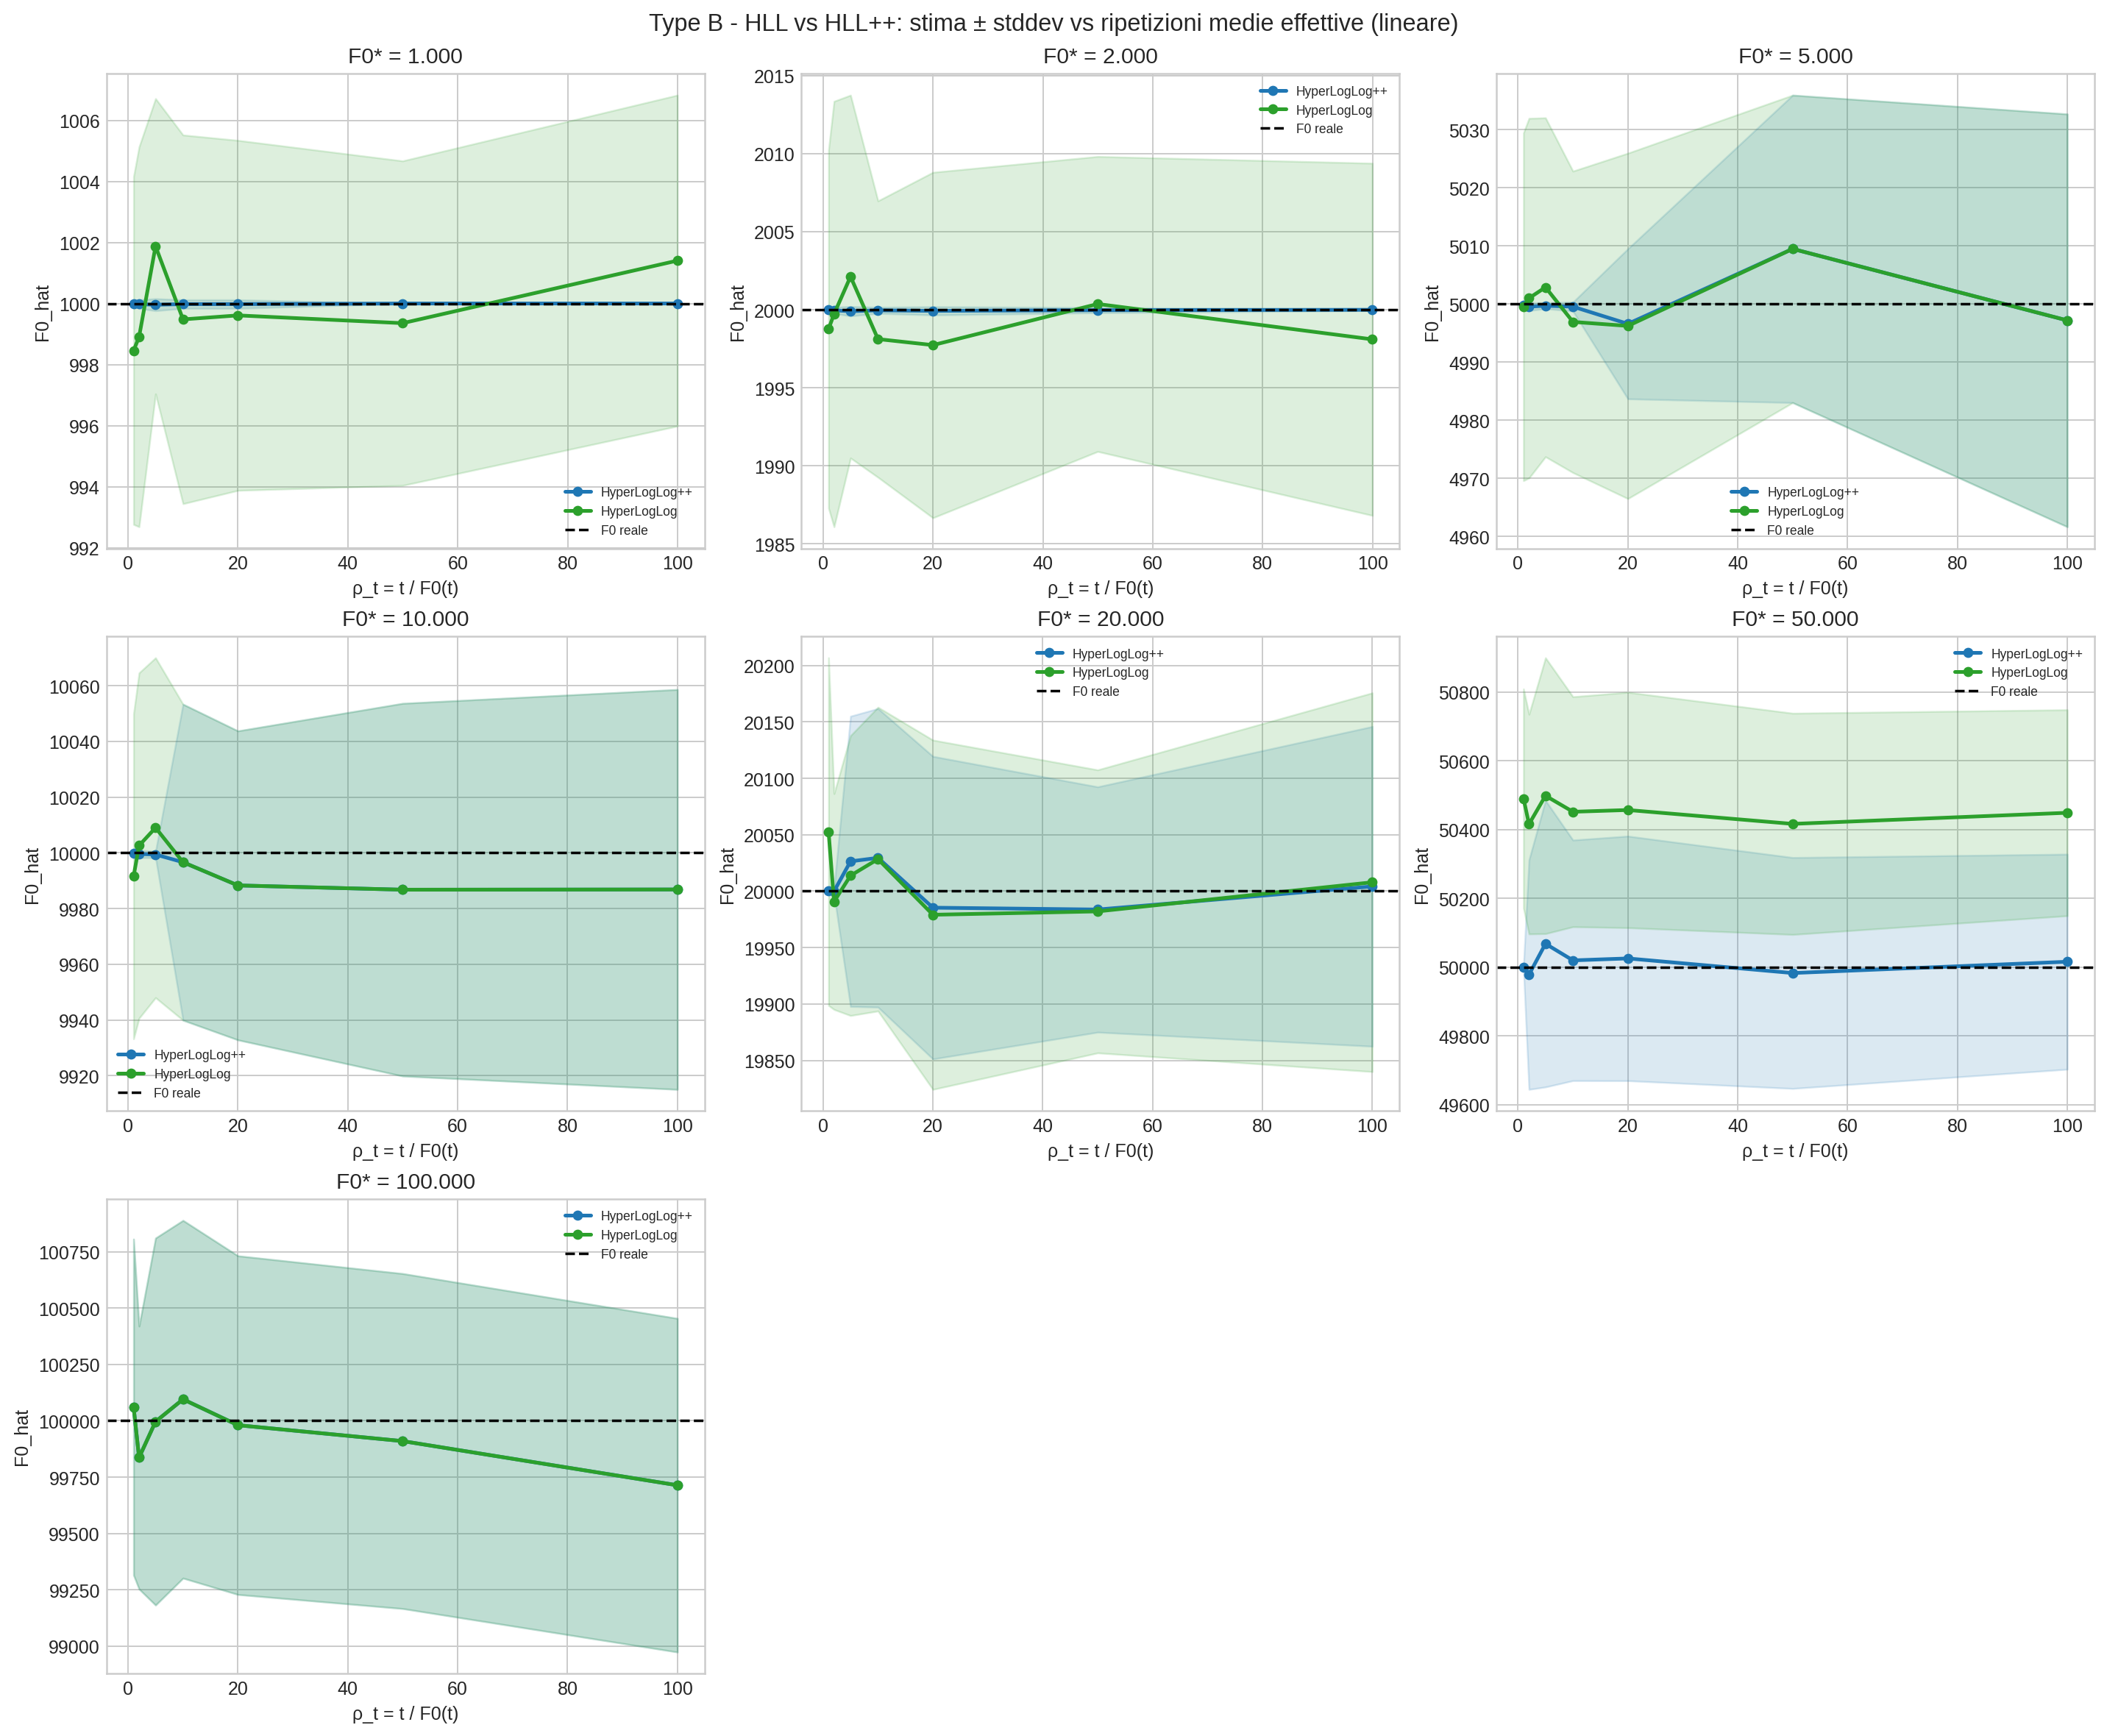
\includegraphics[width=\linewidth]{figures/results/typeB_prefix_constant_rho_hll_hllpp_linear.png}
        \caption{Scala lineare}
        \label{fig:ch5-stream-rho-hll-linear}
    \end{subfigure}
    \hfill
    \begin{subfigure}[t]{0.49\textwidth}
        \centering
        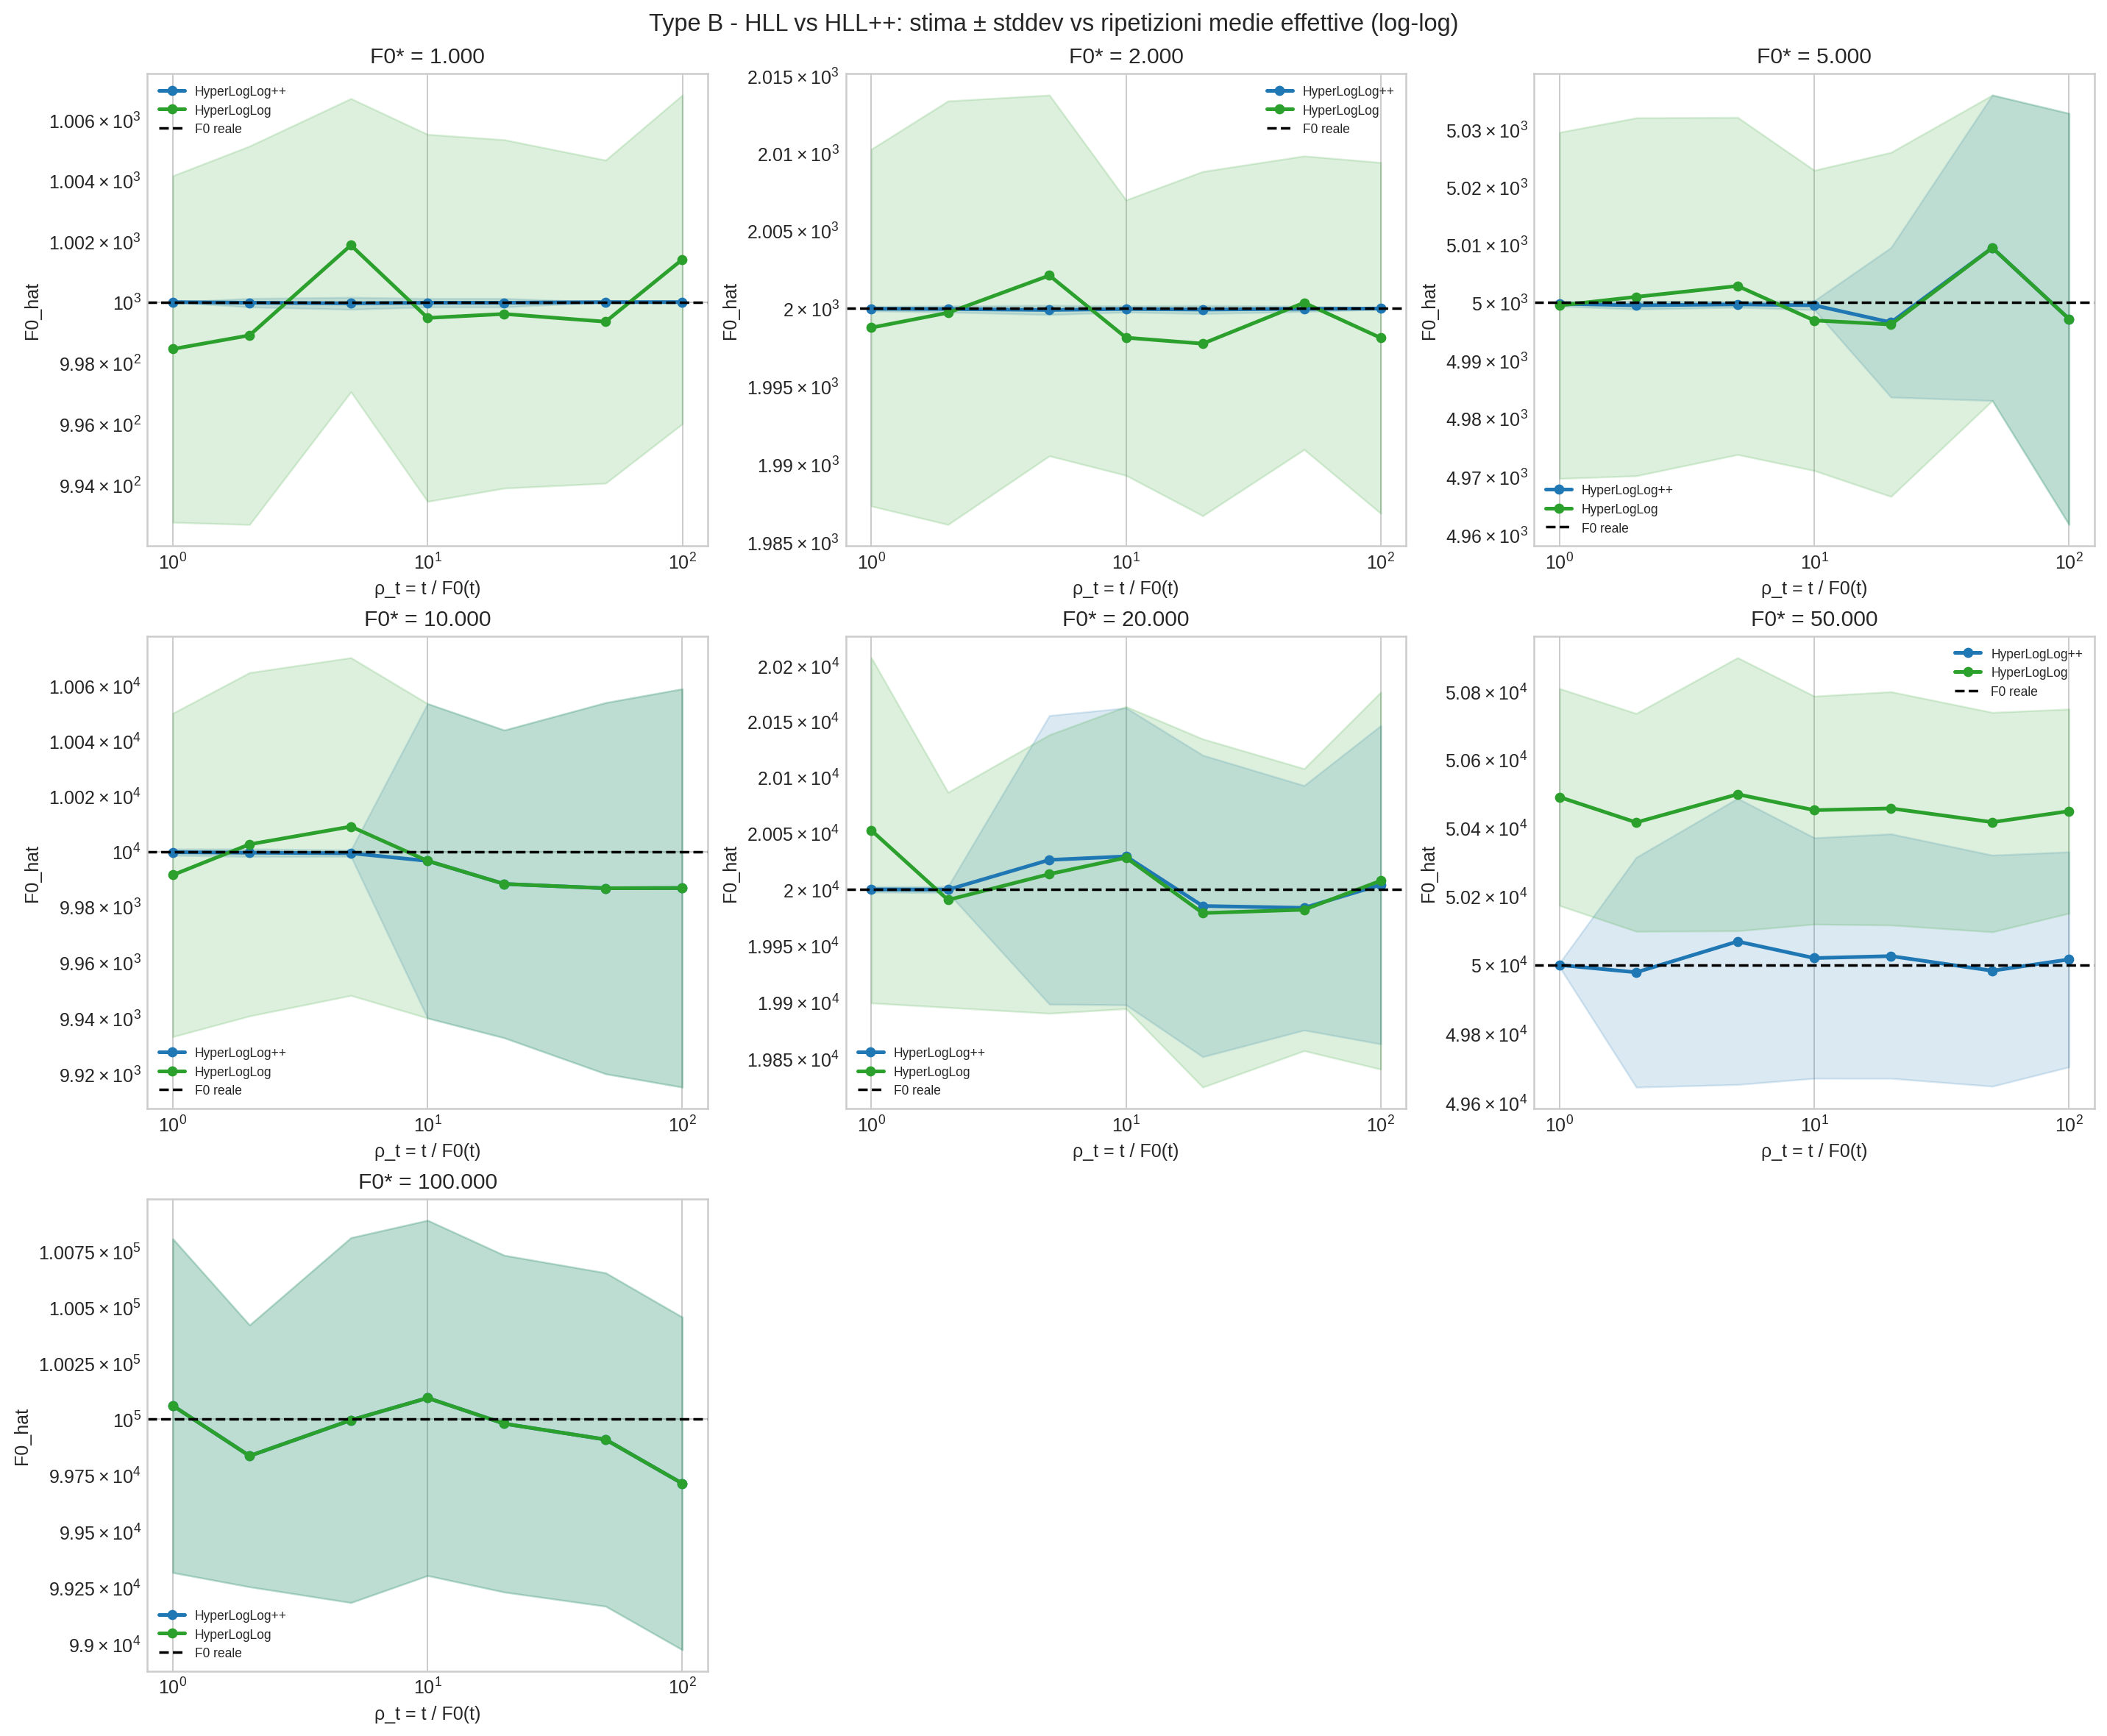
\includegraphics[width=\linewidth]{figures/results/typeB_prefix_constant_rho_hll_hllpp_loglog.png}
        \caption{Scala logaritmica}
        \label{fig:ch5-stream-rho-hll-loglog}
    \end{subfigure}
    \caption{Stima rispetto al rapporto tra elementi processati e distinti, confronto HyperLogLog e HyperLogLog++}
    \label{fig:ch5-stream-rho-hll}
\end{figure}

\subsubsection{Risultati sulla robustezza e sul bias}
Le osservazioni principali emerse dai riassunti ai punti finali osservati sono:
\begin{itemize}
    \item nella vista rispetto alla cardinalità reale del prefisso,
    HyperLogLog e HyperLogLog++ risultano quasi sovrapposti, con errore
    relativo medio ai punti finali di circa \(0.00618\);
    \item nella stessa vista, LogLog segue con errore medio di circa
    \(0.00708\), mentre Probabilistic Counting è nettamente più instabile con
    errore medio di circa \(0.770\);
    \item nella vista rispetto al rapporto tra elementi processati e distinti,
    HyperLogLog++ è l'algoritmo più accurato con errore medio di circa
    \(3.95\cdot 10^{-4}\);
    \item HyperLogLog segue con errore medio di circa \(2.08\cdot 10^{-3}\);
    \item nella stessa vista, Probabilistic Counting ha errore medio di circa
    \(0.346\);
    \item nella seconda vista, l'errore medio più alto è osservato per LogLog,
    con valore di circa \(1.455\).
\end{itemize}

Le Figure~\ref{fig:ch5-stream-f0-hll} e \ref{fig:ch5-stream-rho-hll}
confermano che HyperLogLog++ mantiene il comportamento più stabile nelle due
viste complementari del problema.

\begin{figure}[htbp]
    \centering
    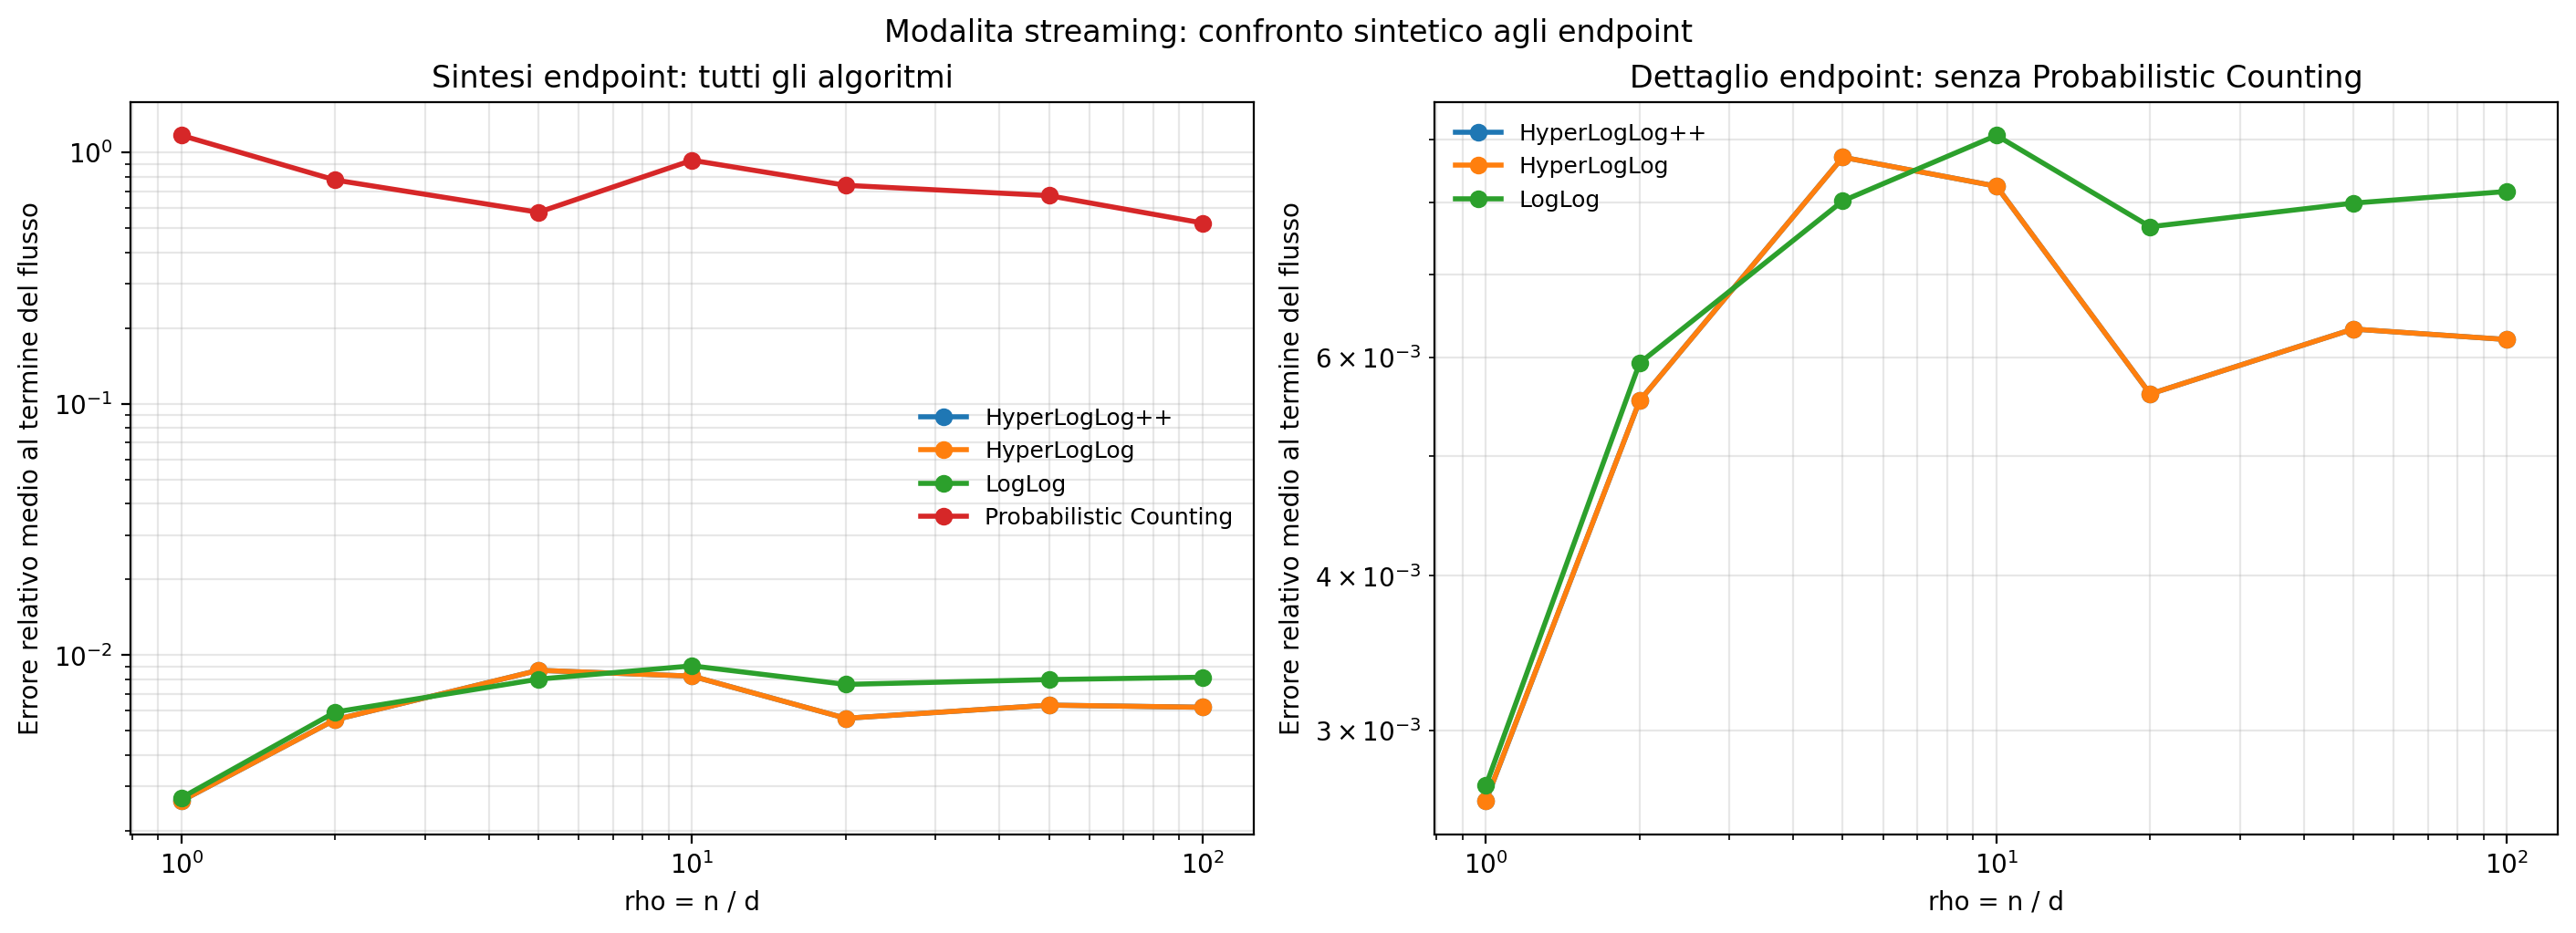
\includegraphics[width=0.98\textwidth]{figures/results/streaming_endpoint_mre_summary.png}
    \caption{Errore relativo medio alla fine della stream. Il pannello sinistro confronta tutti gli algoritmi, mentre quello destro isola HyperLogLog++, HyperLogLog e LogLog}
    \label{fig:ch5-stream-endpoint-summary}
\end{figure}

La Figura~\ref{fig:ch5-stream-endpoint-summary} riassume in forma compatta la
stessa evidenza: Probabilistic Counting resta nettamente separato dagli altri
algoritmi, mentre HyperLogLog++ mantiene il comportamento più regolare e
accurato nel confronto complessivo. Questo risultato è coerente con la
letteratura su HLL++, in cui la riduzione empirica del bias e la gestione
separata dei regimi di cardinalità piccola e intermedia spiegano il vantaggio
rispetto a HLL classico \cite{Heule_Nunkesser_Hall_2013}. Più in generale, i
grafici osservati restano compatibili con la linea evolutiva che porta da
LogLog a HyperLogLog e poi a HyperLogLog++, cioè a una progressiva riduzione
della varianza e del bias pratico
\cite{Durand_Flajolet_2003,Flajolet_Fusy_Gandouet_Meunier_2007,Heule_Nunkesser_Hall_2013}.

\subsection{Analisi sulla variazione dei parametro degli algoritmi}
Per analizzare il comportamento degli algoritmi al variare della precisione, 
\`e necessario isolare l'effetto del parametro.

Di conseguenza, \`e stato fatto un secondo insieme di esperimenti in cui 
sono stati fissati lo stesso insieme di
dati, lo stesso seed e la stessa funzione di hash, variando solo il parametro
interno di ciascun
algoritmo.

L'impostazione scelta per questo esperimento comprende:
\begin{itemize}
    \item l'utilizzo della funzione di hash \texttt{splitmix64}
    \item un seed fissato a \(21041998\)
    \item tre valori rappresentativi per \(\rho \in \{1,10,100\}\)
    \item HyperLogLog++ con \(k \in \{8,10,12,14,16,18\}\)
    \item HyperLogLog e LogLog con \(k \in \{4,6,8,10,12,14,16\}\) e \(L=32\)
    \item Probabilistic Counting con \(L \in \{4,8,12,16,20,24,28,31\}\)
\end{itemize}

Per analizzare il comportamento degli algoritmi al variare della precisione, 
sono stati realizzati due tipi di grafici.

Il primo, tramite una heatmap, riassume l'errore relativo medio alla fine 
del flusso di streaming per ogni coppia di
valori tra \(\rho\) e il parametro dell'algoritmo.

Il secondo sia in scala lineare che in scala logaritmica, fissando $\rho$, mette a confronto la cardinalità reale del flusso 
e la stima, dove ogni retta \`e una diversa precisione dell'algoritmo.
\begin{figure}[htbp]
    \centering
    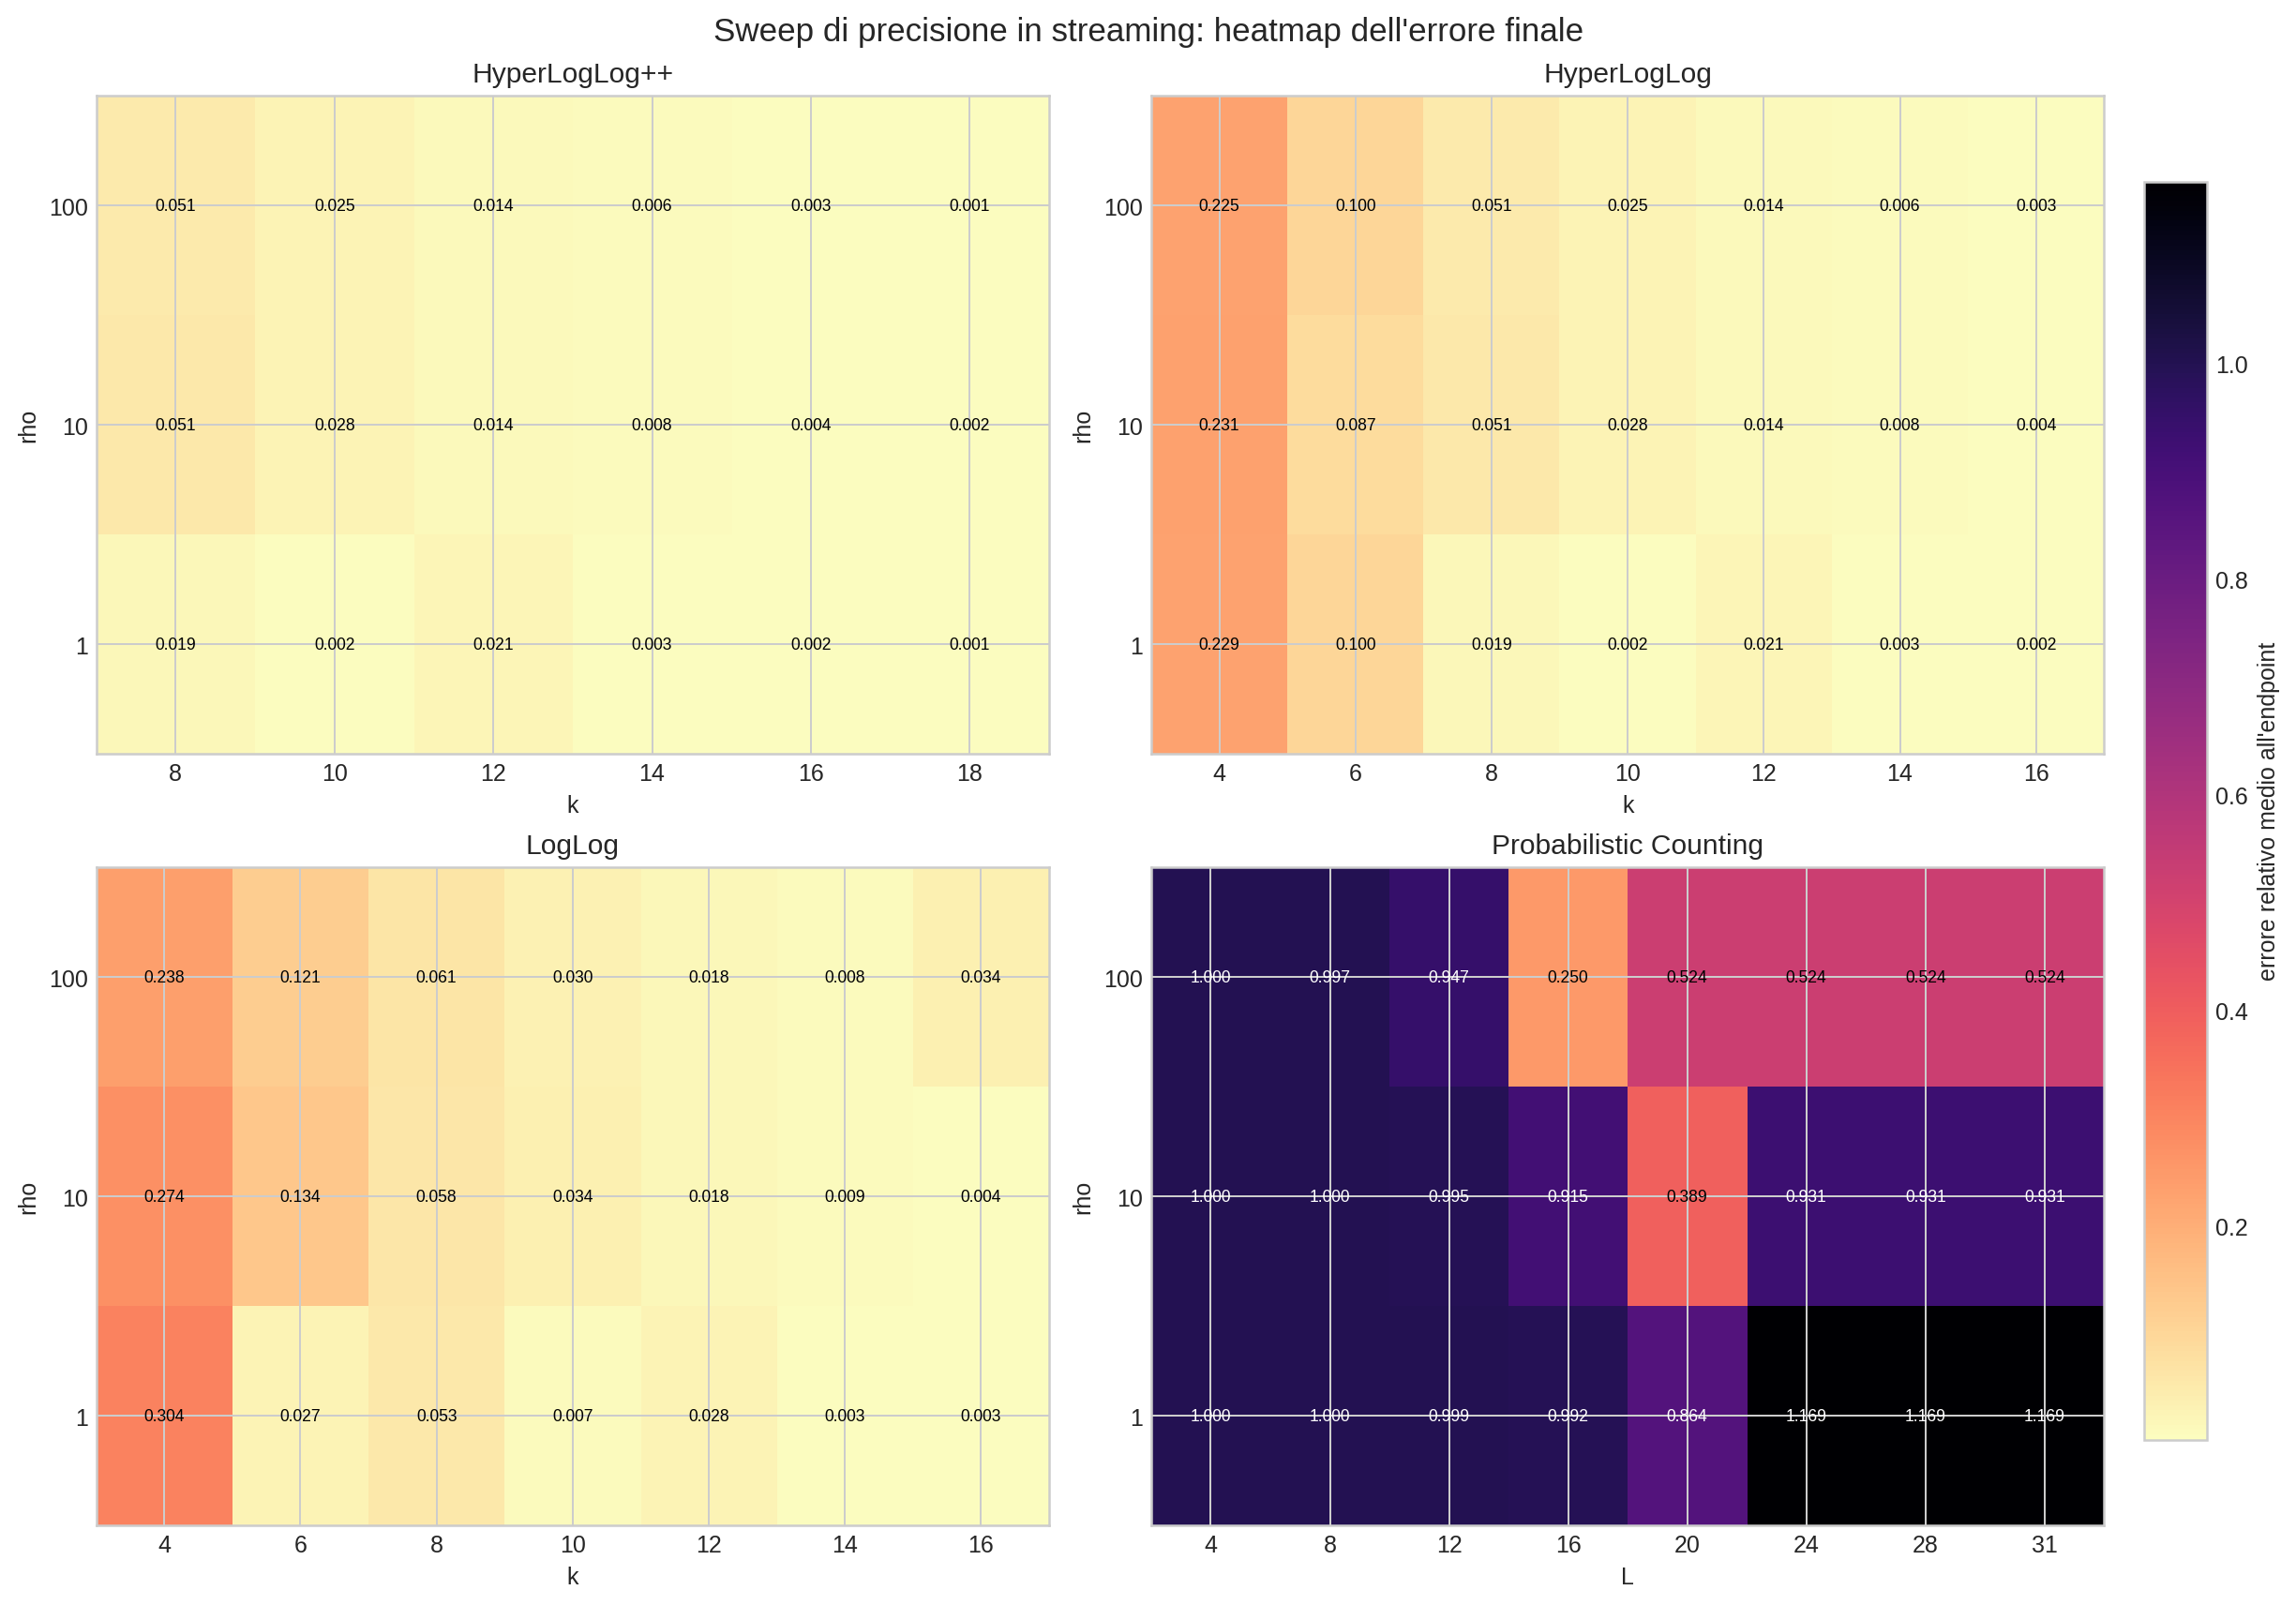
\includegraphics[width=0.98\textwidth]{figures/results/streaming_precision_sweep_endpoint_heatmaps.png}
    \caption{Errore relativo medio alla fine della stream al variare del parametro di precisione e di \(\rho\), per ciascun algoritmo}
    \label{fig:ch5-stream-precision-heatmaps}
\end{figure}

\begin{figure}[p]
    \centering
    \begin{subfigure}[t]{0.49\textwidth}
        \centering
        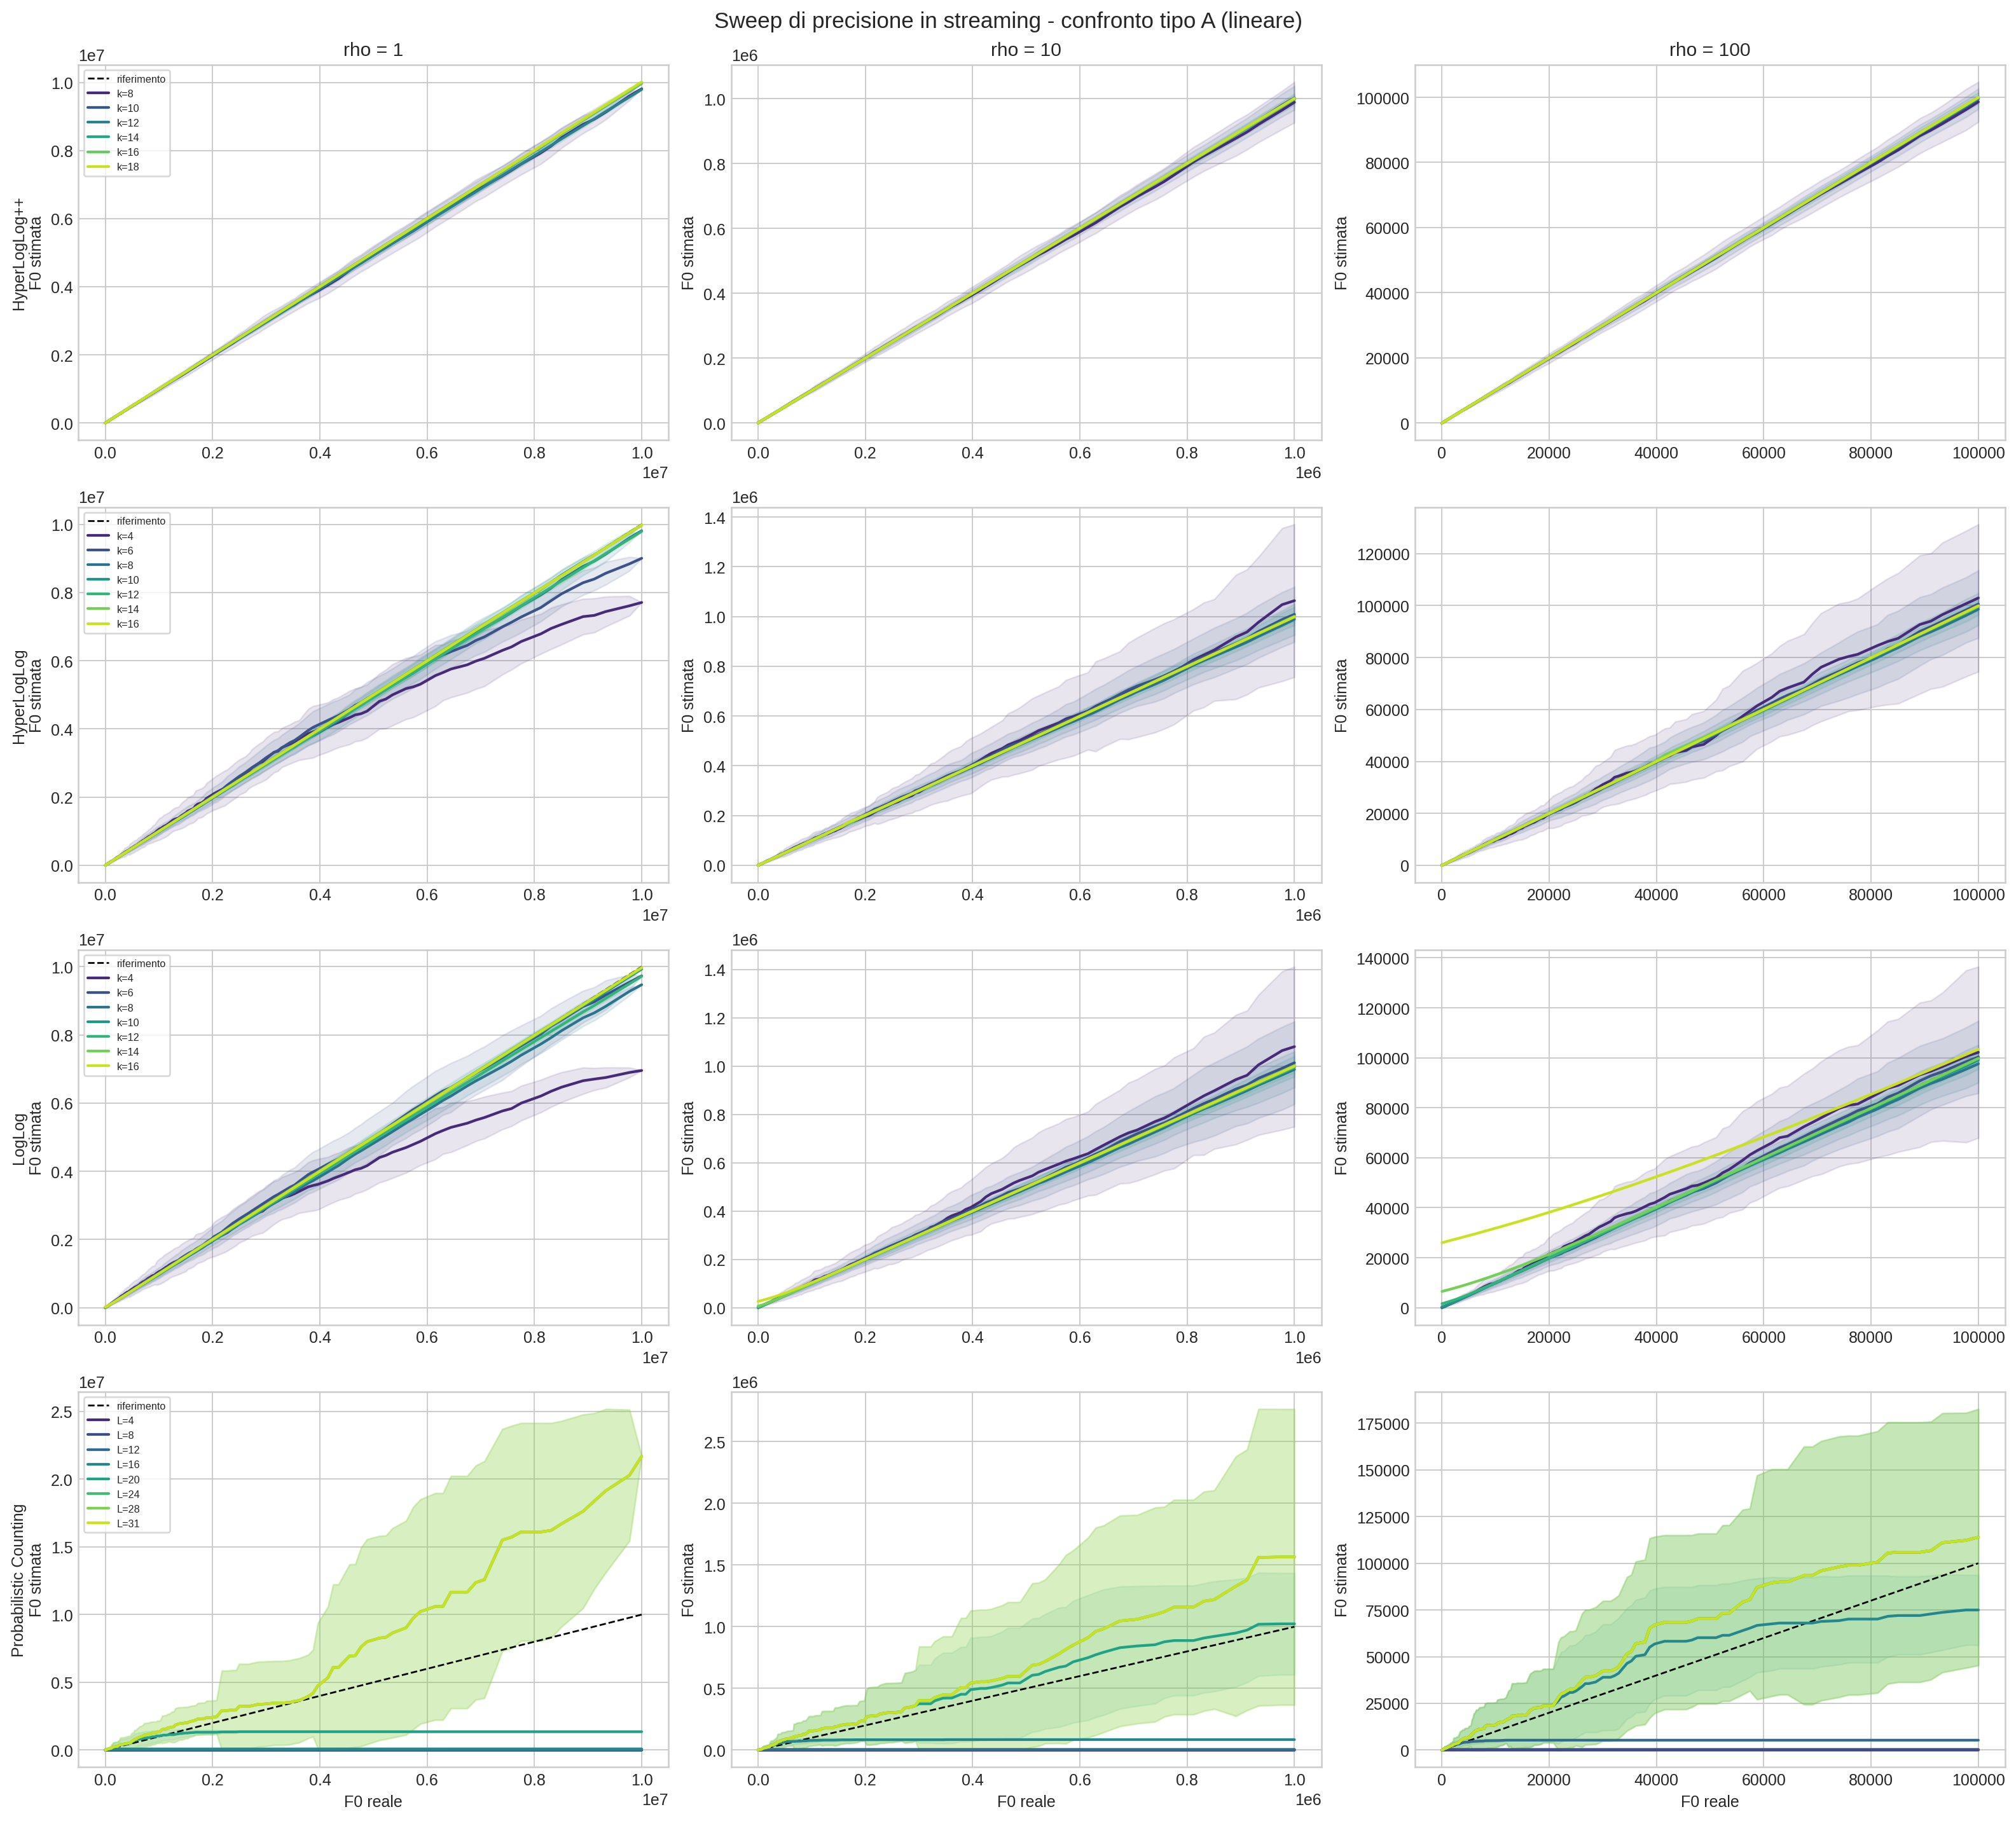
\includegraphics[height=0.33\textheight,keepaspectratio]{figures/results/streaming_precision_sweep_typeA_grid_linear.png}
        \caption{Scala lineare}
        \label{fig:ch5-stream-precision-typea-linear}
    \end{subfigure}
    \hfill
    \begin{subfigure}[t]{0.49\textwidth}
        \centering
        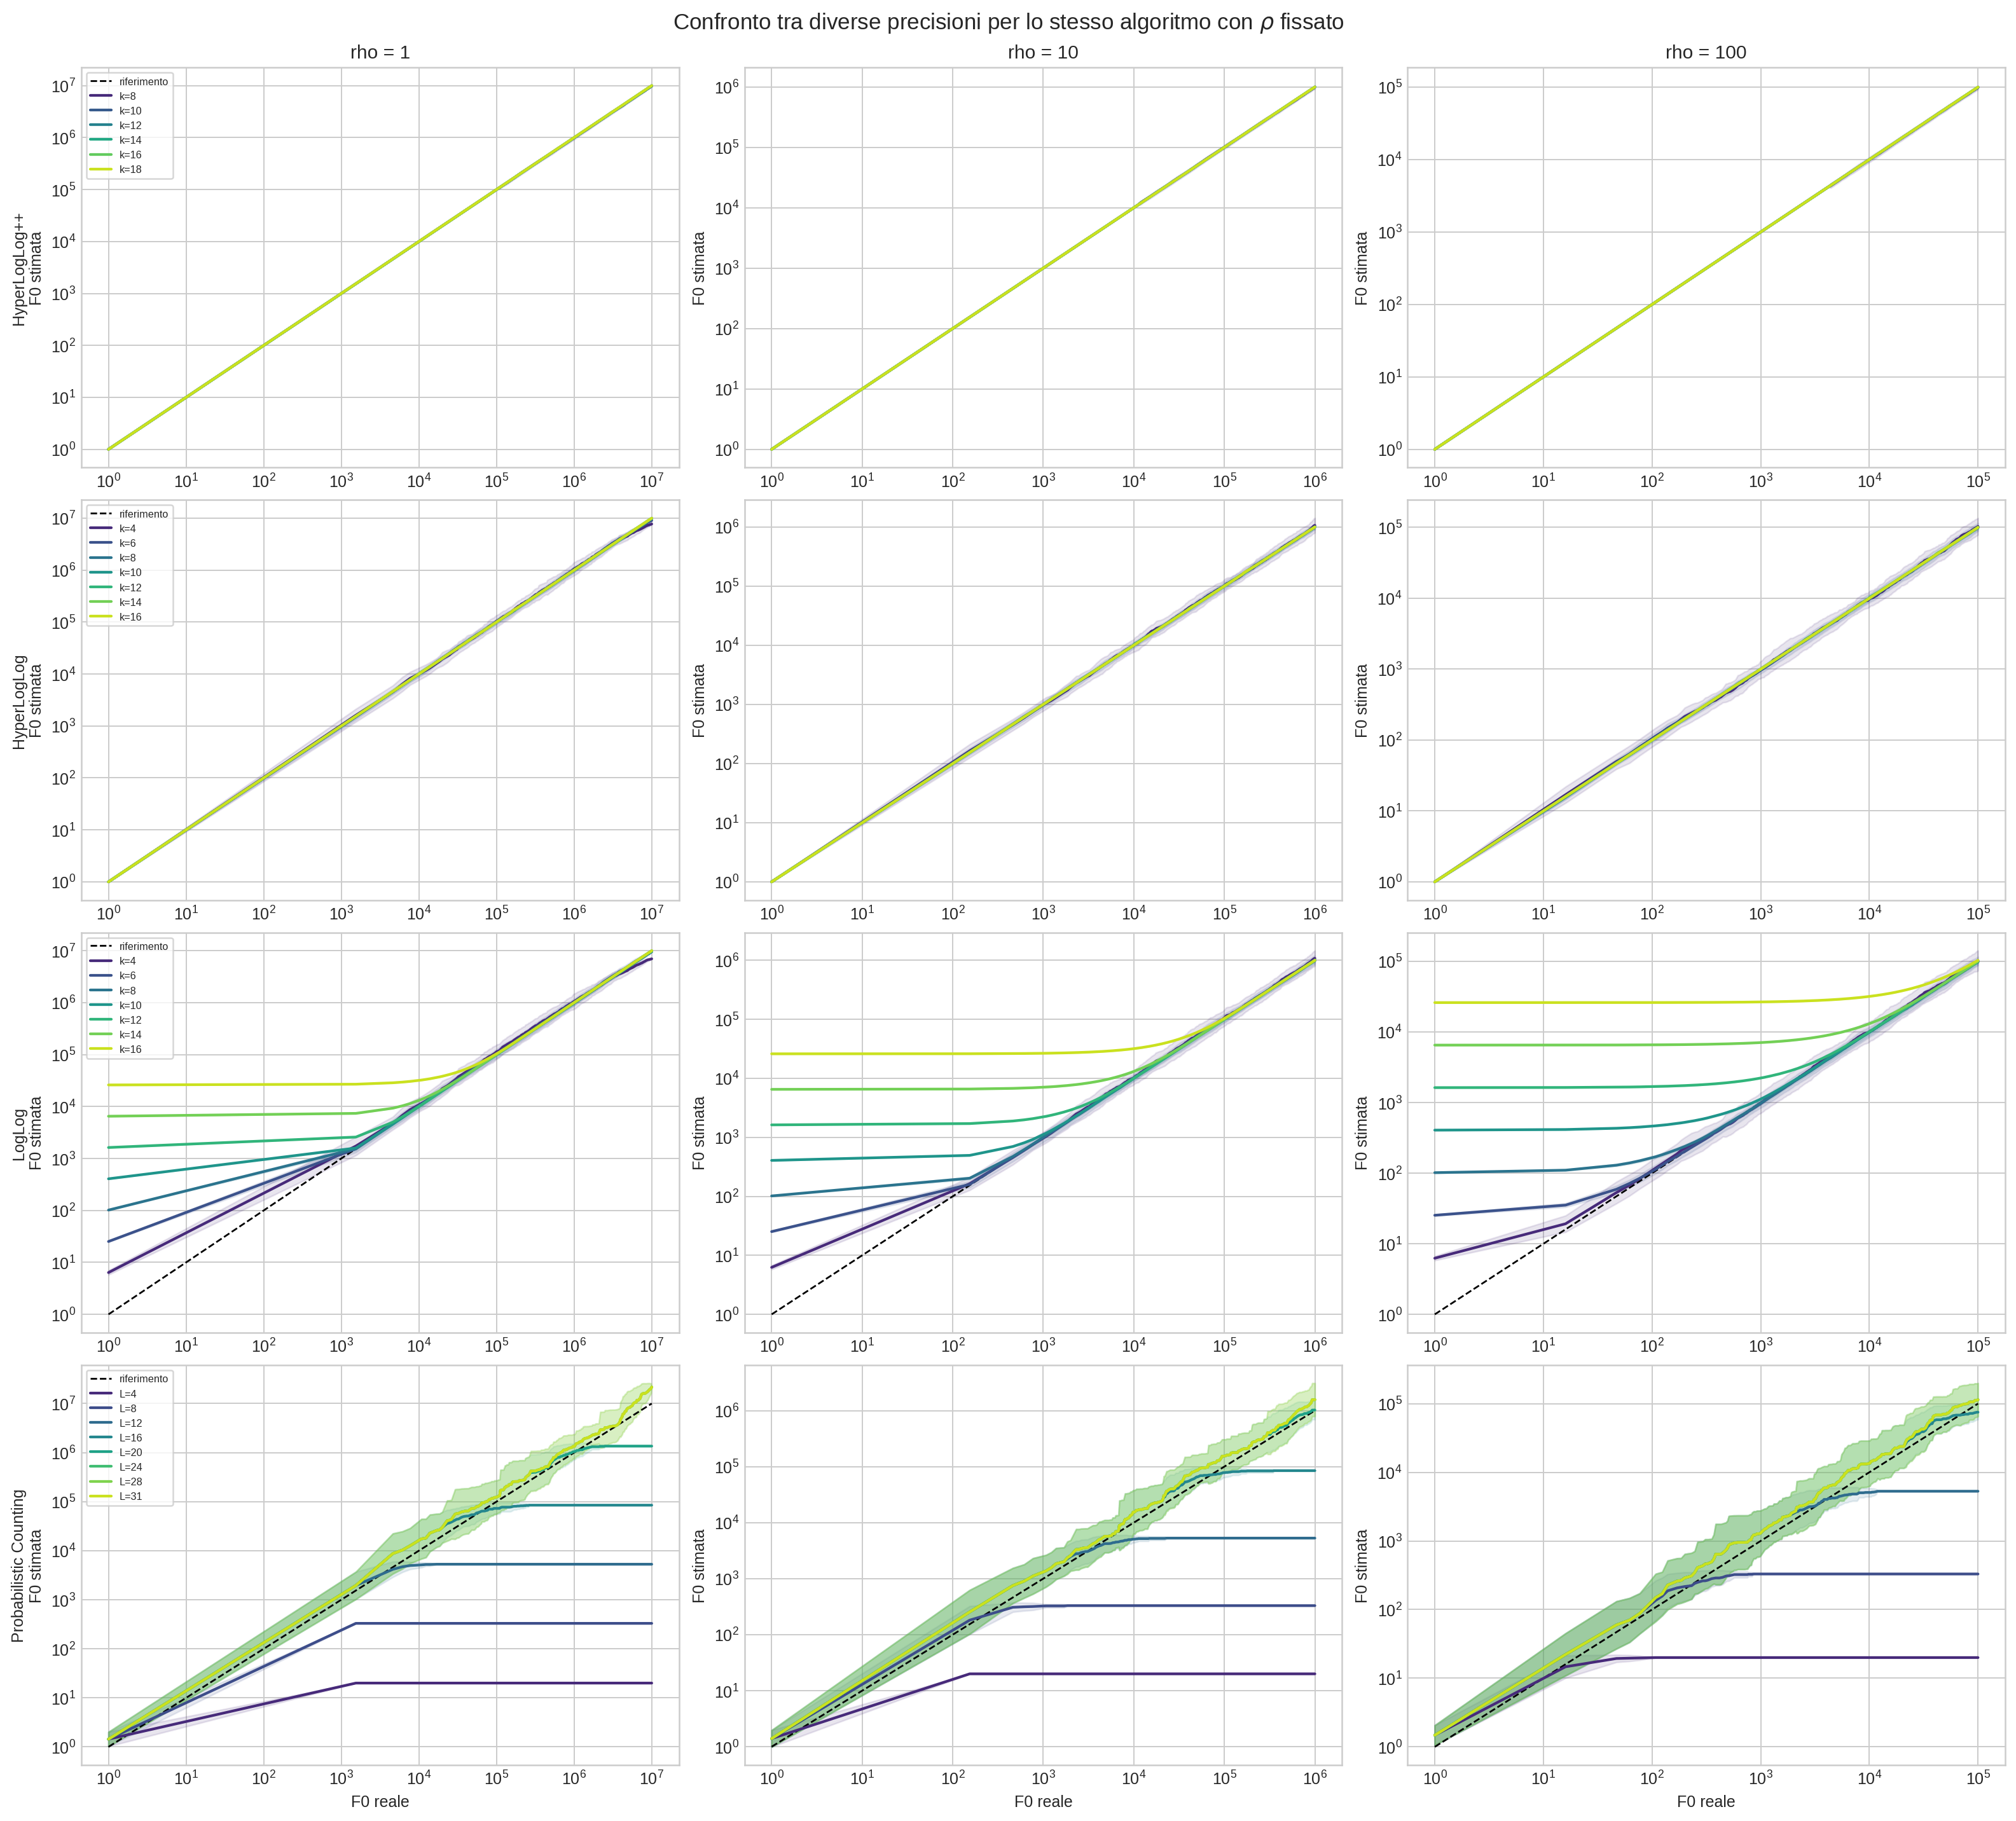
\includegraphics[height=0.33\textheight,keepaspectratio]{figures/results/streaming_precision_sweep_typeA_grid_loglog.png}
        \caption{Scala logaritmica}
        \label{fig:ch5-stream-precision-typea-loglog}
    \end{subfigure}
    \caption{Confronto rispetto alla cardinalità reale del prefisso nell'analisi del parametro di precisione. Le righe corrispondono agli algoritmi e le colonne ai tre valori di \(\rho\)}
    \label{fig:ch5-stream-precision-typea}
\end{figure}

\begin{table}[htbp]
    \centering
    \footnotesize
    \setlength{\tabcolsep}{4pt}
    \renewcommand{\arraystretch}{1.1}
    \begin{tabular}{|l|c|c|c|c|}
        \hline
        Algoritmo & Complessivo & \(\rho=1\) & \(\rho=10\) & \(\rho=100\) \\
        \hline
        HyperLogLog++ & \(k=18\) & \(k=18\) & \(k=18\) & \(k=18\) \\
        \hline
        HyperLogLog & \(k=16\) & \(k=10\) & \(k=16\) & \(k=16\) \\
        \hline
        LogLog & \(k=14\) & \(k=14\) & \(k=16\) & \(k=14\) \\
        \hline
        Probabilistic Counting & \(L=20\) & \(L=20\) & \(L=20\) & \(L=16\) \\
        \hline
    \end{tabular}
    \caption{Miglior parametro osservato per algoritmo nell'analisi del parametro di precisione}
    \label{tab:ch5-stream-precision-best}
\end{table}

\subsubsection{Risultati sulla precisione per ogni algoritmo}

Le Figure~\ref{fig:ch5-stream-precision-heatmaps} e
  \ref{fig:ch5-stream-precision-typea} mostrano che l'aumento del parametro di
  precisione non produce lo stesso effetto per tutti gli algoritmi.

  HyperLogLog++ \`e l'algoritmo con l'andamento pi\`u regolare. Nel dominio
  osservato, all'aumentare di \(k\) l'errore tende a ridursi in modo stabile e il
  valore migliore coincide sempre con \(k=18\), indipendentemente dal valore di
  \(\rho\). Questo comportamento indica che l'algoritmo non solo \`e accurato in
  media, ma risponde anche in modo prevedibile all'aumento delle risorse
  disponibili.

  HyperLogLog mostra una tendenza simile, ma meno uniforme. In media il parametro
  migliore \`e \(k=16\), tuttavia nel caso \(\rho=1\) il beneficio si stabilizza
  gi\`a attorno a \(k=10\). L'aumento del parametro continua quindi a migliorare
  la stima, ma con un guadagno meno regolare rispetto a HyperLogLog++.

  LogLog presenta invece un comportamento pi\`u irregolare. Il parametro migliore
  medio risulta \(k=14\), ma il vantaggio non cresce in modo monotono al crescere
  di \(k\): il valore \(k=16\) migliora il caso intermedio \(\rho=10\), ma non si
  mantiene ottimale negli altri regimi osservati. Questo suggerisce una maggiore
  sensibilit\`a alla scelta del parametro.

  Probabilistic Counting resta nettamente separato dagli altri algoritmi. Anche
  nel caso del parametro migliore, pari a \(L=20\), l'errore finale rimane molto
  pi\`u elevato e il miglioramento ottenuto aumentando \(L\) non \`e sufficiente a
  portare l'algoritmo su livelli comparabili con quelli delle famiglie a
  registri.

Questo esperimento aggiunge quindi un'informazione che i confronti precedenti
non mostravano direttamente. Non basta osservare quale algoritmo sia pi\`u
accurato nel complesso: \`e altrettanto importante capire se la qualit\`a della
stima migliori in modo regolare al variare del parametro. Sotto questo aspetto,
HyperLogLog++ risulta l'algoritmo pi\`u stabile e pi\`u robusto, mentre LogLog e
soprattutto Probabilistic Counting mostrano una dipendenza molto pi\`u marcata
dalla scelta del parametro. Anche questa evidenza è in linea con la dipendenza
classica dell'errore dal numero di registri, che nelle famiglie LogLog e
HyperLogLog segue un andamento dell'ordine di \(1/\sqrt{m}\)
\cite{Durand_Flajolet_2003,Flajolet_Fusy_Gandouet_Meunier_2007}.

\section{Esperimenti sul merge distribuito}
Tutti gli esperimenti sul merge sono stati fatti sull'algoritmo HyperLogLog++. 
Essi sono poi suddivisi secondo tre casi distinti:
\begin{itemize}
    \item \texttt{valid}: merge semanticamente corretto in modo diretto;
    \item \texttt{invalid}: merge non semanticamente corretto;
    \item \texttt{recoverable}: merge non direttamente corretto, ma
    recuperabile con normalizzazione esplicita.
\end{itemize}

La possibilità di costruire sketch locali e combinarli senza rivedere i dati
originari è uno dei motivi principali per cui queste strutture vengono usate in
contesti distribuiti e in sistemi che aggregano grandi collezioni di dataset
\cite{Agarwal_Cormode_Huang_Phillips_Wei_Yi_2012,Ting_2019_BillionsDatasets}.

La sperimentazione del merge omogeneo implementa il caso \texttt{valid}, 
mentre i due esperimenti
eterogenei permettono di osservare separatamente un caso \texttt{invalid} e un
caso \texttt{recoverable}.

 Nella lettura dei risultati eterogenei è utile osservare anche gli scenari
  invertiti tra lato sinistro e lato destro, indicati con il suffisso
  \texttt{rev}. Questa scelta non serve a verificare una nuova proprietà
  algebrica del merge eterogeneo, ma a controllare se il degrado osservato cambi
  quando si scambiano i due contesti locali. La proprietà matematica di
  commutatività del merge è invece già verificata nei test del caso omogeneo,
  insieme all'idempotenza e alla coerenza con il riferimento seriale.

\subsection{Caso omogeneo}
Affinch\'e si possa fare degli esperimenti nel caso di merge omogeneo, \`e
necessario effettuare il merge mantenendo identici la stessa funzione di hash, lo stesso seed
e gli stessi parametri dell'algoritmo.

La configurazione minima scelta prevede:
\[
\rho \in \{1,10,100\},\qquad
k \in \{10,14,18\}
\]
sono state analizzate 36 configurazioni e 900 coppie, combinando i tre valori
di \(k\), i tre regimi di \(\rho\) e le quattro funzioni di hash disponibili.

In tutte le 900 coppie analizzate si osserva:
\[
\Delta_{abs}=0,\qquad \Delta_{rel}=0
\]
La tabella seguente riassume lo stesso risultato nei tre regimi di \(\rho\)
considerati.

\begin{table}[htbp]
    \centering
    \small
    \setlength{\tabcolsep}{6pt}
    \renewcommand{\arraystretch}{1.1}
    \begin{tabular}{|r|r|r|r|r|r|r|}
        \hline
        \(\rho\) & \(d\) & Configurazioni & Coppie totali & Coppie con delta \(\neq 0\) & Max \(\Delta_{abs}\) & Max \(\Delta_{rel}\) \\
        \hline
        1 & \(10^7\) & 12 & 300 & 0 & 0 & 0 \\
        \hline
        10 & \(10^6\) & 12 & 300 & 0 & 0 & 0 \\
        \hline
        100 & \(10^5\) & 12 & 300 & 0 & 0 & 0 \\
        \hline
    \end{tabular}
    \caption{Risultati del controllo omogeneo di HyperLogLog++}
    \label{tab:ch5-merge-homo-summary}
\end{table}

Il controllo omogeneo costituisce il riferimento del caso \texttt{valid} e
mostra che, nel dominio osservato, merge e l'unione seriale coincidono in
modo sistematico. Questo esperimento fornisce quindi la base rispetto alla quale
leggere gli scostamenti osservati nei casi eterogenei. Il risultato è coerente
con la semantica classica del merge per gli sketch HLL-like, che in condizioni
omogenee coincide con lo stato ottenuto processando direttamente l'unione dei
flussi \cite{Ertl_2017_HLLAlgorithms}.

\subsection{Caso eterogeneo}

Nel caso di merge eterogeneo \`e stato deciso
di analizzare due precisi casi distinti. 
Lo scopo di questi esperimenti era cercare di analizzare quanto potesse degradare
il merge in condizioni non ottimali, come ad esempio in un contesto di nodi distribuiti,
in cui ogni nodo aveva a disposizione poca memoria e che fosse necessario utilizzare
precisioni o parametri differenti.

Il primo esperimento consiste nell'analisi sull'utilizzo di funzioni di hash differenti,
che rappresenta un caso \texttt{invalid}, mentre il
merge in caso di precisioni differenti appartiene ai casi \texttt{recoverable} e
richiede quindi una lettura diversa dei risultati.

\subsubsection{Hash mismatch}

  La prima analisi eterogenea riguarda il caso in cui i due sketch vengono
  costruiti usando funzioni di hash differenti, oppure la stessa famiglia di hash
  ma con seed diversi. L'obiettivo è capire come si comporti l'unione di sketch
  quando la semantica dell'hash non è più condivisa tra i due lati.

  Da questo esperimento ci si aspetta sicuramente una degradazione della stima. Poich\'e
  lo stesso numero rappresentato da due funzioni di hash differenti verr\`a rappresentato
  differentemente. L'esperimento vuole vedere quanto effettivamente viene degradata la stima.

  La configurazione considerata è stata:
  \[
  n=10^7,\qquad p=50,\qquad seed=21041998,\qquad
  d\in\{10^5,10^6,10^7\}
  \]
  da cui si ricava
  \[
  \rho\in\{100,10,1\}
  \]
  con precisione fissata a \(k=14\).

  Le funzioni di hash considerate in questa configurazione minima sono
  \texttt{splitmix64}, \texttt{xxhash64}, \texttt{murmurhash3} e
  \texttt{siphash24}. Gli scenari osservati sono sette:
  \begin{itemize}
      \item \texttt{ctrl}: controllo omogeneo locale, con la stessa funzione di
      hash sui due lati e seed del dataset su entrambi;
      \item \texttt{seed\_xx} e \texttt{seed\_xx\_rev}: stessa hash
      \texttt{xxhash64}, ma seed diversi nei due lati;
      \item \texttt{seed\_murmur} e \texttt{seed\_murmur\_rev}: stessa hash
      \texttt{murmurhash3}, ma seed diversi nei due lati;
      \item \texttt{family} e \texttt{family\_rev}: confronto tra
      \texttt{xxhash64} e una funzione di hash diversa tra
      \texttt{splitmix64}, \texttt{murmurhash3} e \texttt{siphash24}.
  \end{itemize}

  I casi di \emph{seed mismatch} sono stati testati solo su
  \texttt{xxhash64} e \texttt{murmurhash3}, perché in questa configurazione minima sono
  le due famiglie per cui l'utilizzo di seed differenti è stato usato come fattore
  di eterogeneità. Nei casi \texttt{family} e \texttt{family\_rev}, invece,
  l'eterogeneità riguarda direttamente l'utilizzo di funzioni di hash.

  Lo scenario \texttt{ctrl} è presente anche in questo esperimento come
  riferimento locale nella stessa figura e nella stessa tabella. Non rappresenta
  un esperimento distinto dal caso omogeneo discusso in precedenza, ma un suo
  sottoinsieme su HyperLogLog++ con \(k=14\), utile per confrontare direttamente
  i casi \texttt{invalid} con il comportamento corretto.

  Nel controllo omogeneo la strategia usata è \texttt{direct}. Nei casi
  \texttt{invalid}, invece, vengono osservate due strategie:
  \texttt{reject} e \texttt{unsafe\_naive\_merge}. La prima non produce una stima
  di merge e registra esplicitamente il caso incompatibile. La seconda forza il
  merge come se la coppia fosse compatibile, ed è quindi usata come controllo
  negativo sperimentale.

   Questo controllo serve quindi a distinguere i casi in cui il merge è trattato
  come semanticamente valido dai casi in cui viene forzato esplicitamente come
  controllo negativo.

  L'esperimento copre 1800 righe complessive, distribuite su 72 file in formato
  CSV:
  \begin{itemize}
      \item 300 coppie nel controllo omogeneo;
      \item 750 coppie \texttt{invalid} con \texttt{reject};
      \item 750 coppie \texttt{invalid} con \texttt{unsafe\_naive\_merge}.
  \end{itemize}

  La Figura~\ref{fig:ch5-hash-mismatch} mostra, per i diversi valori di \(\rho\),
  il contrasto tra il merge omogeneo locale e il merge forzato nei casi
  \texttt{invalid}. La Tabella~\ref{tab:ch5-hash-mismatch-summary} ne riassume i
  principali valori numerici. Le quantità \(\overline{\varepsilon}_{merge}\) e
  \(\overline{\varepsilon}_{serial}\) indicano rispettivamente l'errore relativo
  medio del merge e del riferimento seriale. La colonna finale riporta invece il
  degrado medio, cioè la media del rapporto punto per punto tra errore del merge
  ed errore del riferimento seriale.

  \begin{table}[htbp]
      \centering
      \small
      \setlength{\tabcolsep}{5pt}
      \renewcommand{\arraystretch}{1.1}
      \begin{tabular}{|l|r|r|r|r|r|}
          \hline
          Scenario & Coppie & \(\overline{\varepsilon}_{merge}\) & \(\overline{\varepsilon}_{serial}\) &
  \(\max \varepsilon_{merge}\) & Degrado medio \\
          \hline
          \texttt{ctrl} & 300 & 0.006233 & 0.006233 & 0.025913 & 1.00 \\
          \hline
          \texttt{seed\_xx} & 75 & 0.342374 & 0.007436 & 0.969548 & 49.45 \\
          \hline
          \texttt{seed\_xx\_rev} & 75 & 0.343830 & 0.010076 & 0.969548 & 28.82 \\
          \hline
          \texttt{seed\_murmur} & 75 & 0.347522 & 0.004836 & 0.984223 & 206.46 \\
          \hline
          \texttt{seed\_murmur\_rev} & 75 & 0.348319 & 0.004606 & 0.984223 & 307.18 \\
          \hline
          \texttt{family} & 225 & 0.352037 & 0.007436 & 1.009634 & 50.36 \\
          \hline
          \texttt{family\_rev} & 225 & 0.352802 & 0.005832 & 1.009634 & 130.76 \\
          \hline
      \end{tabular}
      \caption{Risultati del merge eterogeneo con funzioni di hash differenti}
      \label{tab:ch5-hash-mismatch-summary}
  \end{table}

    \begin{figure}[htbp]
      \centering
      \begin{subfigure}[t]{0.98\textwidth}
          \centering
          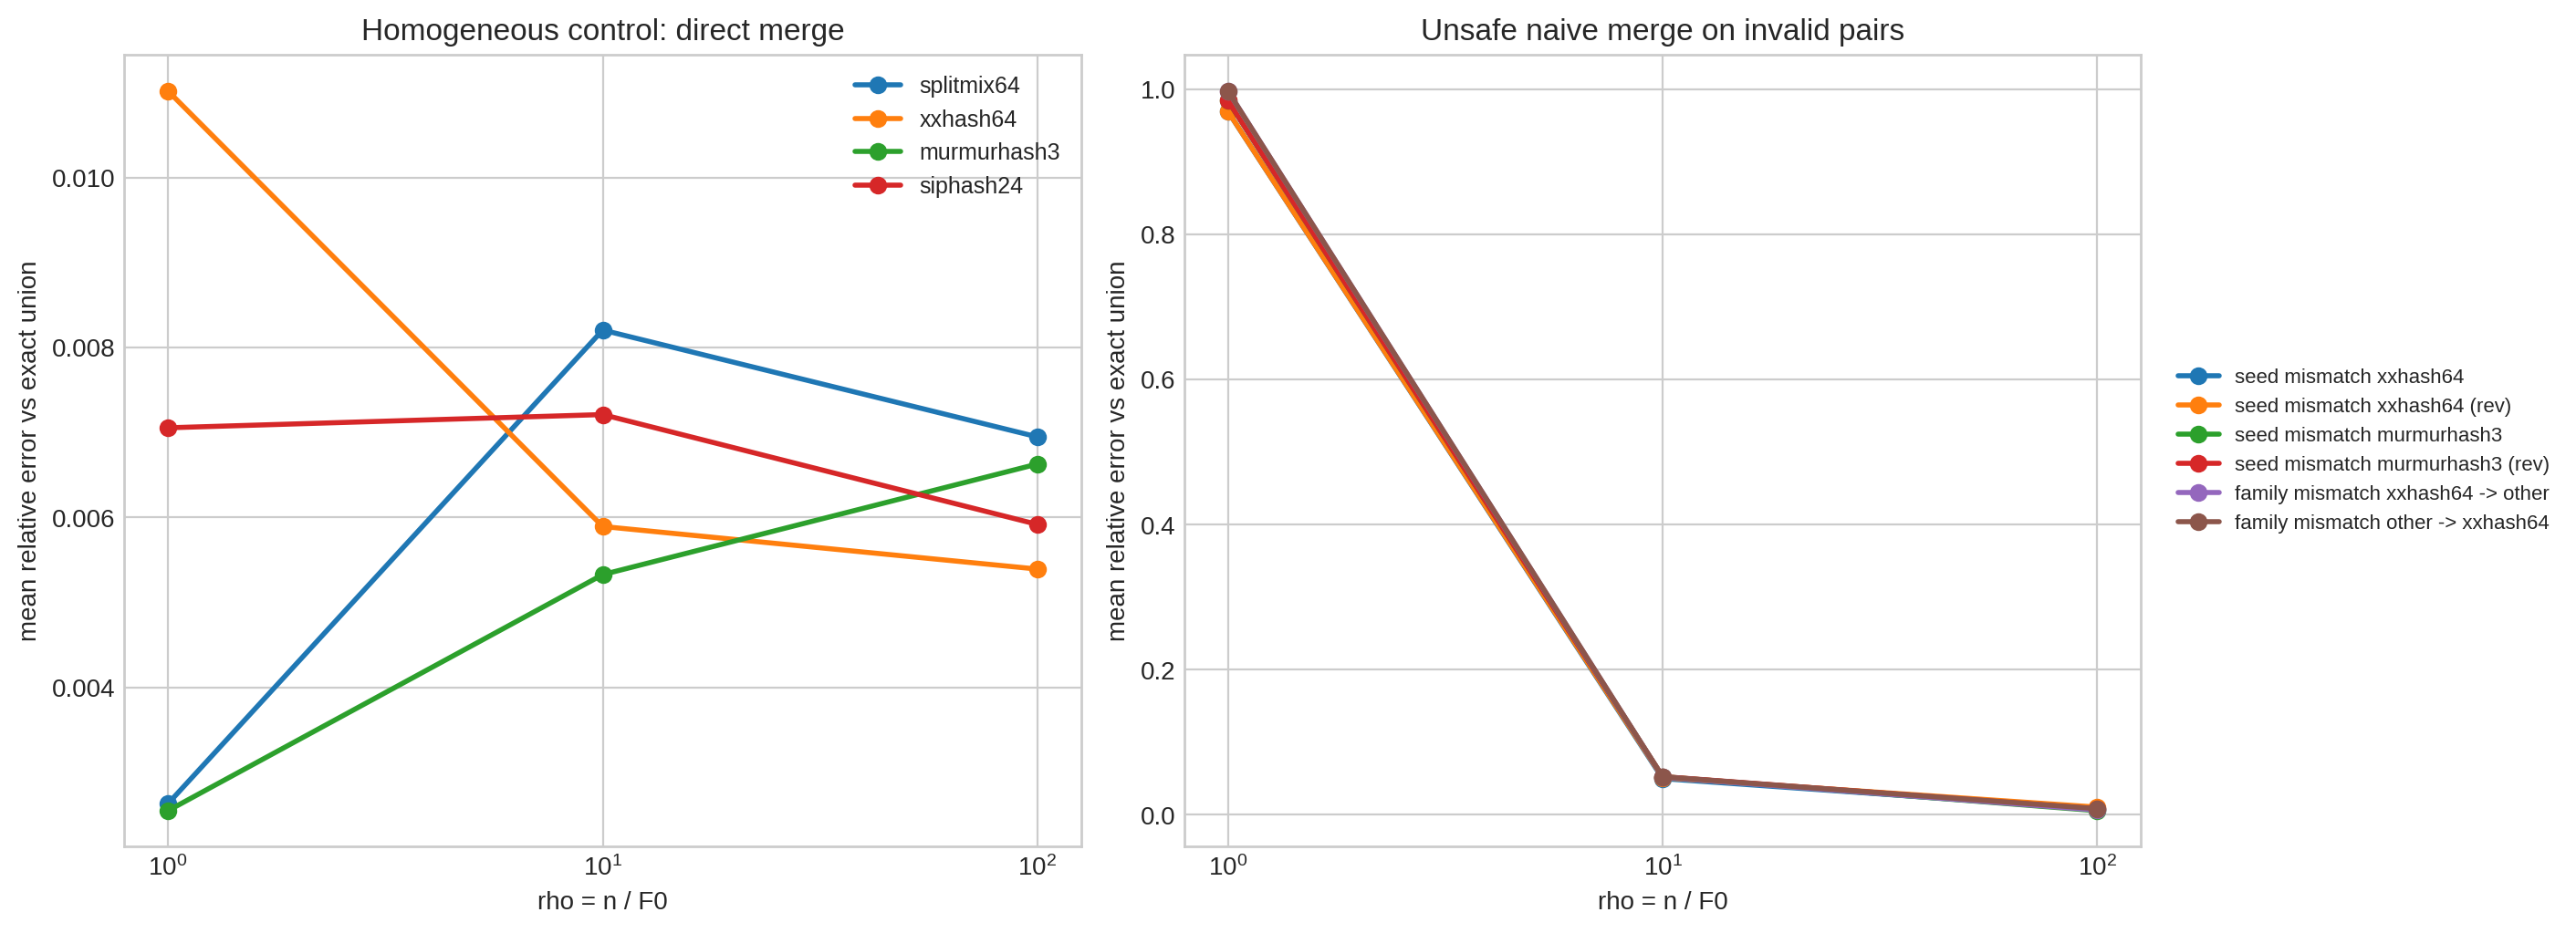
\includegraphics[width=\linewidth]{figures/results/merge_hpp_hash_mismatch_overview.png}
          \caption{Controllo omogeneo e andamento medio del merge forzato nei casi \texttt{invalid}}
          \label{fig:ch5-hash-mismatch-overview}
      \end{subfigure}
      \caption{Esperimento di merge eterogeneo con funzioni di hash differenti}
      \label{fig:ch5-hash-mismatch}
  \end{figure}

  Dai risultati emerge che, nei casi \texttt{invalid}, il merge forzato produce un
  degrado netto rispetto al riferimento seriale e conferma che l'eterogeneità
  dell'hash rompe la semantica comune necessaria al merge. Nel regime più
  critico, \(\rho=1\), l'errore relativo medio raggiunge valori prossimi o
  superiori a 1, con massimo pari a 1.009634. La strategia \texttt{reject}, al
  contrario, evita di trattare queste coppie come merge validi e mantiene nel
  protocollo sperimentale soltanto la stima seriale e l'unione esatta.

\subsubsection{Precision mismatch}

  La seconda analisi eterogenea riguarda l'esperimento in cui la funzione di hash resta
  costante, ma i due sketch vengono costruiti con precisioni differenti, cio\`e con parametri differenti
  per l'algoritmo, in questo caso cambia la quantit\`a di registri utilizzati.

  L'obiettivo è capire se l'utilizzo di parametri differenti rende il merge
  direttamente invalido oppure se il caso possa essere recuperato tramite una
  normalizzazione esplicita.

  La configurazione considerata è stata:
  \[
  n=10^7,\qquad p=50,\qquad seed=21041998,\qquad
  d\in\{10^5,10^6,10^7\}
  \]
  da cui si ricava
  \[
  \rho\in\{100,10,1\}
  \]
  con funzione di hash fissata a \texttt{xxhash64} e seed di hash identico sui
  due lati, pari a \(21041998\).

  Le coppie di precisione osservate sono:
  \[
  (k_{left},k_{right}) \in
  \{(10,14),(14,10),(10,18),(18,10),(14,18),(18,14)\}
  \]
  Questi sei casi vengono letti in tre gruppi di precisione:
  \texttt{10 vs 14}, \texttt{10 vs 18} e \texttt{14 vs 18}, ciascuno osservato
  nelle due direzioni tra lato sinistro e lato destro.

  In tutti questi casi la coppia è classificata come \texttt{recoverable}. Per
  questa ragione vengono osservate tre strategie:
  \texttt{reject}, \texttt{unsafe\_naive\_merge} e
  \texttt{reduce\_then\_merge}. La prima non produce una stima di merge e
  registra esplicitamente il caso. La seconda forza il merge senza alcuna
  normalizzazione preventiva. La terza riduce entrambi gli sketch alla precisione
  più bassa compatibile e applica poi il merge nello spazio comune.

  Questo controllo serve quindi a distinguere i casi in cui il parametro di precisione \`e differente
e che venga trattato come merge recuperabile dai casi in cui il
  merge viene forzato senza normalizzazione.

  L'esperimento copre 1350 righe complessive, distribuite su 54 file in formato
  CSV:
  \begin{itemize}
      \item 450 coppie \texttt{recoverable} con \texttt{reject};
      \item 450 coppie \texttt{recoverable} con \texttt{unsafe\_naive\_merge};
      \item 450 coppie \texttt{recoverable} con \texttt{reduce\_then\_merge}.
  \end{itemize}

  La Tabella~\ref{tab:ch5-precision-mismatch-summary} riassume i principali
  valori numerici dell'esperimento. Le quantità
  \(\overline{\varepsilon}_{merge}\) e \(\overline{\varepsilon}_{serial}\)
  indicano rispettivamente l'errore relativo medio del merge e del caso
  seriale. Anche in questo caso l'ultima colonna riporta il degrado medio, cioè
  la media del rapporto punto per punto tra errore del merge ed errore del
  merge seriale. La riga \texttt{reject} non corrisponde a una stima di
  merge, ma a una strategia di rifiuto; per questo le colonne relative al merge
  restano non valorizzate.

  \begin{table}[htbp]
      \centering
      \small
      \setlength{\tabcolsep}{5pt}
      \renewcommand{\arraystretch}{1.1}
      \begin{tabular}{|l|r|r|r|r|r|}
          \hline
          Strategia & Coppie & \(\overline{\varepsilon}_{merge}\) & \(\overline{\varepsilon}_{serial}\) & \(\max
  \varepsilon_{merge}\) & Degrado medio \\
          \hline
          \texttt{reject} & 450 & -- & 0.016651 & -- & -- \\
          \hline
          \texttt{unsafe\_naive\_merge} & 450 & 0.363882 & 0.016651 & 1.061378 & 32.37 \\
          \hline
          \texttt{reduce\_then\_merge} & 450 & 0.016651 & 0.016651 & 0.057418 & 1.00 \\
          \hline
      \end{tabular}
      \caption{Risultati del merge eterogeneo nel caso in cui i parametri degli algoritmi non coincidono}
      \label{tab:ch5-precision-mismatch-summary}
  \end{table}

  \begin{figure}[htbp]
      \centering
      \begin{subfigure}[t]{0.98\textwidth}
          \centering
          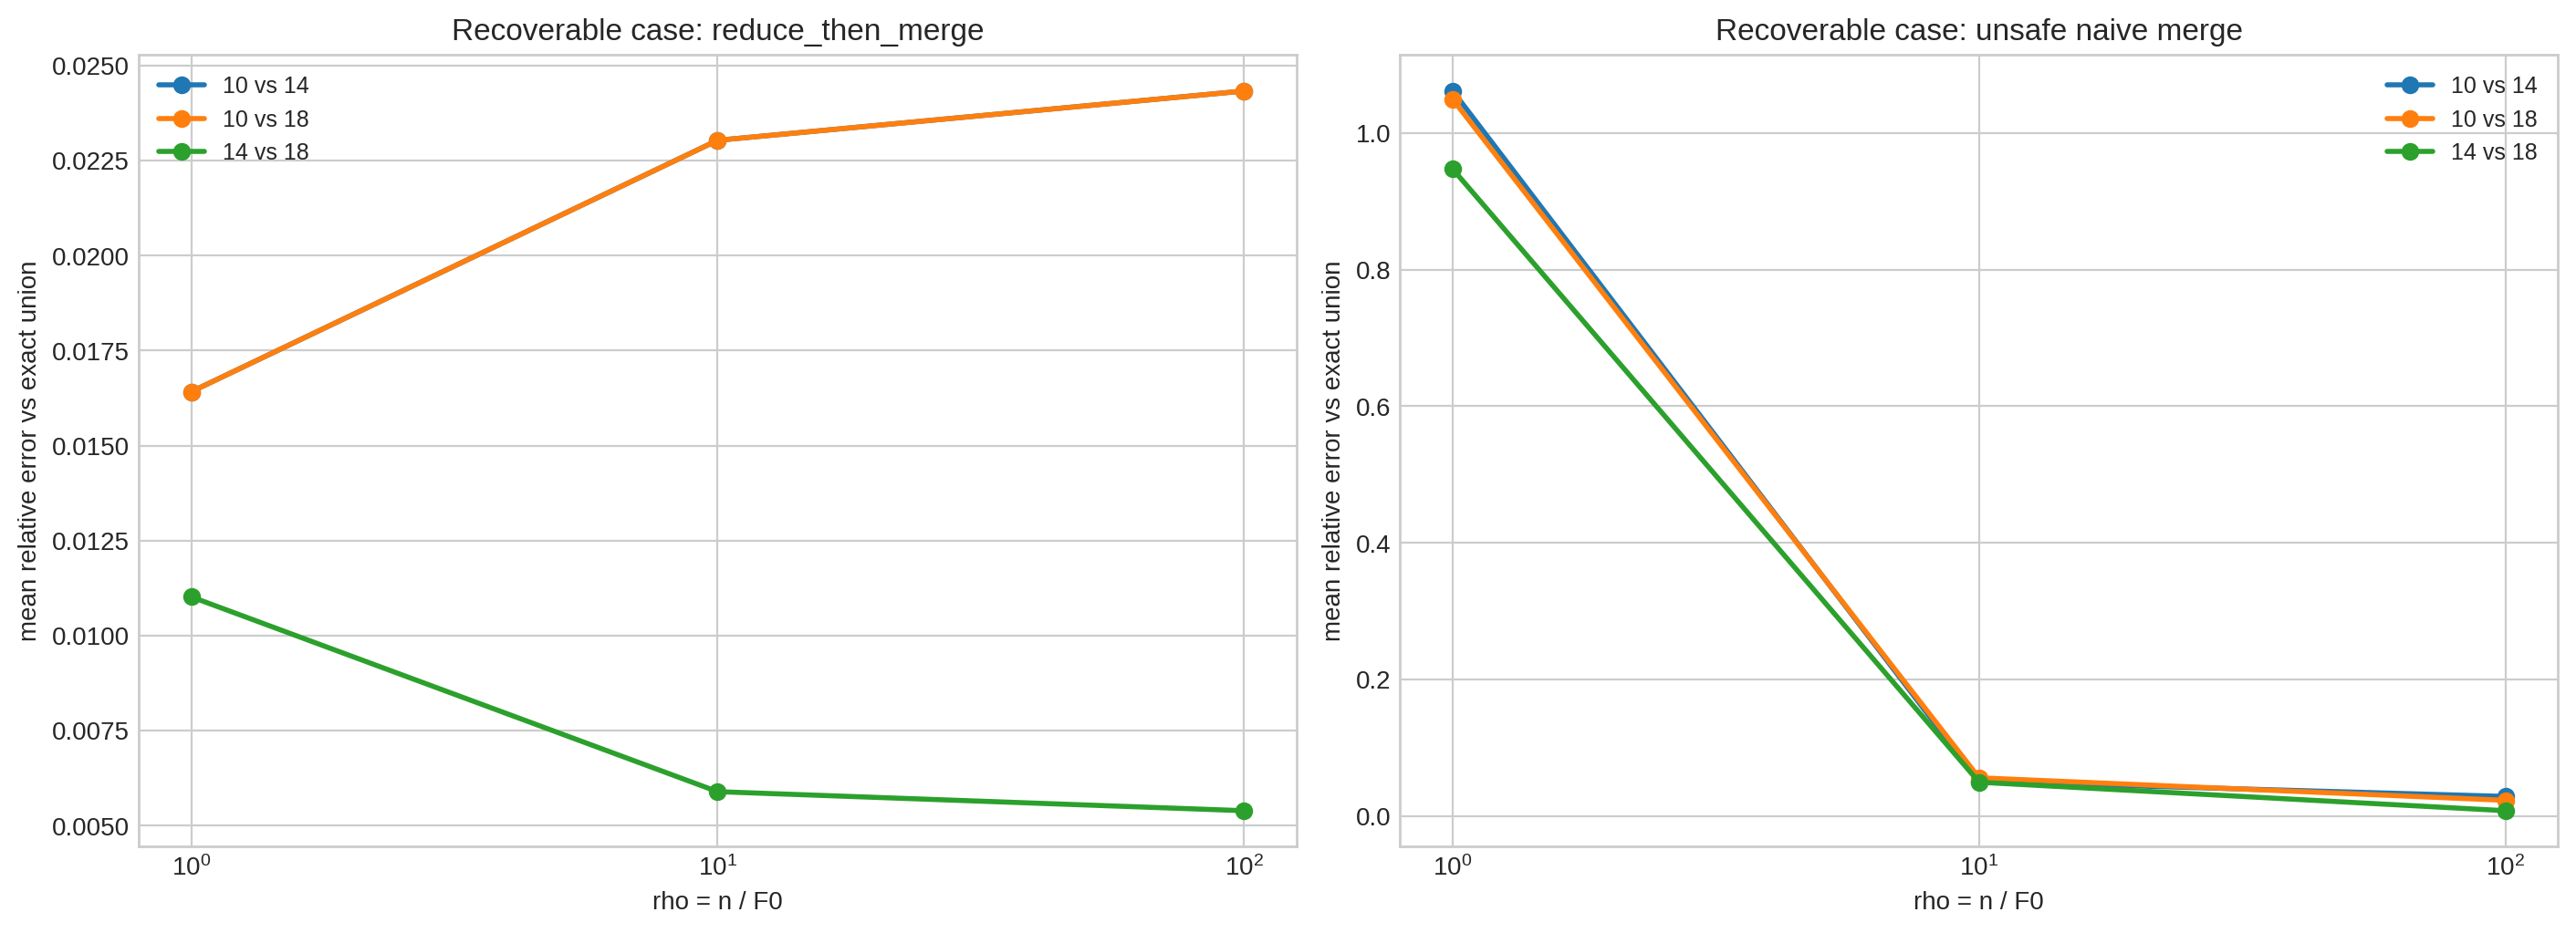
\includegraphics[width=\linewidth]{figures/results/merge_hpp_precision_mismatch_overview.png}
          \caption{Confronto tra \texttt{reduce\_then\_merge} e \texttt{unsafe\_naive\_merge} nel caso in cui i parametri degli algoritmi non coincidono}
          \label{fig:ch5-precision-mismatch-overview}
      \end{subfigure}
  \end{figure}

  \paragraph{Correttezza della normalizzazione \texttt{reduce\_then\_merge}}

  Dai risultati emerge che, nei casi \texttt{recoverable}, la normalizzazione alla
  precisione minima elimina lo scostamento introdotto dall'utilizzo di parametri differenti. 
  Con l'utilizzo della strategia \texttt{reduce\_then\_merge}, il comportamento coincide infatti
  sia con il riferimento seriale sia con il riferimento omogeneo alla precisione
  più bassa, con degrado medio pari a \(1.00\). Questo comportamento è coerente
  con la letteratura più recente sugli sketch HyperLogLog, che tratta la
  riduzione alla precisione minima come passaggio corretto per rendere
  confrontabili sketch costruiti con parametri diversi
  \cite{Ertl_2017_HLLAlgorithms}.

  \paragraph{Degrado del merge forzato nel caso \texttt{recoverable}}

  Quando la normalizzazione non viene applicata, il merge forzato mostra invece un
  degrado netto rispetto al riferimento seriale. Nel gruppo \texttt{10 vs 14},
  l'errore relativo medio passa da circa \(0.0290\) per \(\rho=100\) a
  \(0.0509\) per \(\rho=10\), fino a raggiungere \(1.061378\) per \(\rho=1\).
  Nel gruppo \texttt{10 vs 18} i valori sono molto simili, con massimo
  \(1.049045\) nel regime \(\rho=1\). Nel gruppo \texttt{14 vs 18} il degrado
  resta più contenuto per \(\rho=100\), ma cresce nuovamente fino a
  \(0.947067\) quando \(\rho=1\). Anche in questo caso, quindi, il merge forzato
  non si limita a introdurre una perdita moderata di accuratezza, mentre la
  strategia \texttt{reduce\_then\_merge} riporta il comportamento al riferimento
  corretto.

\section{Risultati ottenuti}

I risultati presentati in questo capitolo possono essere riassunti in quattro
punti principali.

\begin{itemize}
    \item \textbf{Algoritmo migliore: HyperLogLog++.} Nel dominio sperimentale
    osservato, HyperLogLog++ risulta il metodo migliore perché combina
    \textit{accuratezza media più alta}, \textit{minore dispersione della
    stima} e \textit{comportamento più regolare al variare del parametro di
    precisione}. Le Figure~\ref{fig:ch5-stream-f0-hll},
    \ref{fig:ch5-stream-rho-hll} e
    \ref{fig:ch5-stream-endpoint-summary} mostrano infatti che HyperLogLog++
    mantiene la stima più stabile sia rispetto alla cardinalità reale del
    prefisso sia rispetto al rapporto tra elementi processati e distinti. La
    Tabella~\ref{tab:ch5-stream-precision-best} conferma inoltre che, durante l'esperimento sui possibili parametri,
    HyperLogLog++ è anche l'algoritmo con la risposta più
    prevedibile all'aumentare di \(k\), con valore migliore osservato sempre pari
    a \(k=18\).

    \item \textbf{Coincidenza tra merge omogeneo e riferimento seriale.} Quando
    due sketch condividono la stessa funzione di hash, lo stesso seed e gli
    stessi parametri, il merge coincide con il caso seriale nel dominio
    osservato. La Tabella~\ref{tab:ch5-merge-homo-summary} riporta infatti
    \(\Delta_{abs}=0\) e \(\Delta_{rel}=0\) in tutte le coppie analizzate.
    Questo è il risultato di riferimento del caso \texttt{valid} e mostra che,
    in condizioni omogenee, il merge preserva correttamente la semantica dello
    sketch.

    \item \textbf{Hash diverse nel merge compromettono la correttezza.} Quando
    i due sketch sono costruiti con funzioni di hash diverse, oppure con seed
    diversi della stessa famiglia di hash, il merge produce un degrado
    netto rispetto al riferimento seriale. La
    Tabella~\ref{tab:ch5-hash-mismatch-summary} mostra che l'errore relativo
    medio del merge cresce di oltre un ordine di grandezza e, nel regime più
    critico \(\rho=1\), può superare il valore \(1\). Questo conferma che il
    merge richiede non solo lo stesso algoritmo, ma anche una semantica comune
    dell'hash.

    \item \textbf{La tecnica \texttt{reduce\_then\_merge} recupera il caso di
    precisioni diverse.} Se i due sketch usano la \textit{stessa funzione di
    hash} ma \textit{precisioni diverse}, il merge non è direttamente corretto,
    ma può essere recuperato normalizzando entrambi gli sketch alla precisione
    minima comune prima dell'unione. La
    Tabella~\ref{tab:ch5-precision-mismatch-summary} mostra che, con
    \texttt{reduce\_then\_merge}, l'errore medio del merge coincide con quello
    del riferimento seriale e del corrispondente caso omogeneo, mentre il merge
    senza normalizzazione introduce un degrado netto.
\end{itemize}

Complessivamente, il risultato principale del capitolo è che HyperLogLog++
emerge come il miglior stimatore tra quelli implementati, mentre sul lato del
merge la correttezza dipende in modo decisivo dalla compatibilità semantica tra
gli sketch: il caso omogeneo coincide con il seriale, l'eterogeneità dell'hash
rompe la correttezza, e quando due sketch hanno precisioni diverse il merge resta recuperabile solo
attraverso una normalizzazione esplicita.
